\documentclass[11pt]{article}

\usepackage{amsmath,amssymb}
\usepackage{booktabs}
\usepackage{geometry}
\usepackage{graphicx}
\usepackage{hyperref}
\usepackage[numbers,sort&compress]{natbib}
\usepackage{xurl}

\geometry{margin=1in}
\graphicspath{{plots/}{../plots/}{./}}
\hypersetup{colorlinks=true,linkcolor=blue,citecolor=blue,urlcolor=blue}

\title{Lyman-$\alpha$ forest $P_{1\mathrm{D}}$\\[0.35em]
\large Part II. Jeans smoothing, small-scale density,\\
three-dimensional flux power, and the Arinyo-i-Prats comparison}
\author{Helena}
\date{2 November 2026}

\begin{document}
\maketitle

\begin{abstract}
This note specifies the extensions of the Lyman-$\alpha$ $P_{1\mathrm{D}}$ calculator after the discussion of 13~October 2026.
The linear matter spectrum, the Kaiser projection, and the optical-depth sightlines of Part~I are retained without modification.
A Jeans factor may multiply a stored matter spectrum before either flux path is evaluated.
On that screened spectrum the calculation compares a Gaussian density contrast with a lognormal density, measures both the Kaiser and the sightline flux power at small scales, and quantifies the sampling noise of the sightline estimator as the ensemble grows from $256$ to $10\,000$ lines.
The flux spectra are then repeated at $z=5$ out to $k_\parallel=0.2\,\mathrm{s\,km}^{-1}$.
Finally, $P_F(k,\mu)$ is measured in one periodic Gaussian volume after a lognormal optical-depth map and a linear line-of-sight velocity, and compared with the Kaiser formula of Part~I and with the nonlinear fitting formula of Arinyo-i-Prats et al.\ at the parameter values published for their fiducial hydrodynamic simulation.
Every equation is stated with its source, and every operation is assigned to the function that implements it.
\end{abstract}

\section{Relation to Part I}
\label{sec:relation}

Part~I constructs the linear cold-dark-matter spectrum $P_\mathrm{CDM}$ from the Eisenstein--Hu transfer function \citep{Eisenstein:1997ik}, forms the three-dimensional flux power
\begin{equation}
\label{eq:kaiser}
P_F(k,\mu)
=
b_F^{2}\,(1+\beta_F\mu^{2})^{2}\,P_\mathrm{CDM}(k),
\qquad
\mu=\frac{k_\parallel}{k},
\end{equation}
with fixed $b_F=-0.14$ and $\beta_F=1.4$ \citep{Kaiser:1987qv,McDonald:2001fe,Gordon:2023dua}, and integrates over transverse modes to obtain
\begin{equation}
\label{eq:p1d}
P_{1\mathrm{D}}(k_\parallel)
=
\int_{k_\parallel}^{k_\mathrm{max}}
\frac{k\,\mathrm{d}k}{2\pi}\,
P_F\!\left(k,\mu=\frac{k_\parallel}{k}\right).
\end{equation}
Independently, Part~I draws periodic Gaussian lines from the isotropic projection of $P_\mathrm{CDM}$, maps them to a lognormal density \citep{Coles:1991if,Bi:1996fh},
\begin{equation}
\label{eq:lognormal}
\Delta=\exp\!\left(\delta_G-\tfrac12\mathrm{Var}(\delta_G)\right),
\end{equation}
and assigns a fluctuating Gunn--Peterson optical depth \citep{Gunn:1965hd,Hui:1997dp}
\begin{equation}
\label{eq:fgpa}
\beta=2-0.7\,(\gamma-1),
\qquad
\tau=A\Delta^{\beta},
\qquad
F=e^{-\tau},
\end{equation}
with $\gamma=1.5$ so that $\beta=1.65$, solving for $A$ so that $\langle F\rangle=0.80$.
The fiducial cosmology is unchanged:
\begin{equation}
\Omega_m=0.31,\quad
\Omega_b=0.049,\quad
h=0.67,\quad
n_s=0.965,\quad
A_s=2.1\times 10^{-9}.
\end{equation}
Figures~09--12 and~14 are at $z=3$. Figure~13 is at $z=5$.
The entry points \texttt{p1d\_skm} and \texttt{run\_fgpa\_skewers} continue to default to an unsmoothed spectrum.

The six requests of 13~October were: (i)~spectra out to $k\sim 0.2\,\mathrm{s\,km}^{-1}$ at $z\sim 5$; (ii)~a larger ensemble, as a test that the sightline scatter falls; (iii)~a three-dimensional realisation from which $P_F(k,\mu)$ is measured; (iv)~a comparison of that measurement with the nonlinear model of Arinyo-i-Prats et al.\ \citep{Arinyo-i-Prats:2015vqa}; (v)~a Gaussian pressure filter; (vi)~a lognormal description of weakly nonlinear dark matter.
Sections~\ref{sec:jeans}--\ref{sec:noise} address (v), (vi), the small-scale flux at $z=3$, and (ii).
Section~\ref{sec:z5} addresses (i).
Section~\ref{sec:box} addresses (iii) and (iv).
Section~\ref{sec:code} assigns every operation to code and states how the figures are produced.

\section{Jeans factor}
\label{sec:jeans}

The pressure smoothing added here is the multiplicative cutoff used by Arya et al.\ in their lognormal forest model \citep{Arya:2022uke},
\begin{equation}
\label{eq:jeans}
P_\mathrm{CDM}(k)
\to
P_\mathrm{CDM}(k)\,\exp(-2 x_J^{2} k^{2}),
\end{equation}
with $k$ in $h\,\mathrm{Mpc}^{-1}$ and $x_J$ in comoving $\mathrm{Mpc}/h$.
The two lengths examined are
\begin{equation}
x_J = 0.10\,\mathrm{Mpc}/h = 100\,\mathrm{kpc}/h,
\qquad
x_J = 0.05\,\mathrm{Mpc}/h = 50\,\mathrm{kpc}/h.
\end{equation}
At fixed $k$ the exponent is proportional to $x_J^{2}$, so $100\,\mathrm{kpc}/h$ removes more power than $50\,\mathrm{kpc}/h$.
The identity $x_J=0$ recovers the Part~I spectrum at every $k$.

Equation~\eqref{eq:jeans} multiplies the three-dimensional matter spectrum before any line is drawn and before the integral \eqref{eq:p1d} is evaluated.
The pixel-space Gaussian filters of Part~I, one for pressure and one for thermal broadening, remain in the sightline code and are left at zero width in every figure of this part.
The gas density is still the lognormal map \eqref{eq:lognormal} of the filtered linear field.

\section{Three-dimensional spectra from the Kaiser expression}
\label{sec:3d}

Figure~\ref{fig:jeans3d} has two panels, both at $z=3$.
The left panel is $P_\mathrm{CDM}(k)$ for $x_J=0$, $0.10$, and $0.05\,\mathrm{Mpc}/h$.
The three curves overlie from the largest scales through about $1\,h\,\mathrm{Mpc}^{-1}$.
Beyond that wavenumber the $100\,\mathrm{kpc}/h$ curve falls first, then the $50\,\mathrm{kpc}/h$ curve.
The unsmoothed curve is the Eisenstein--Hu spectrum of Part~I.
On the stored table, direct evaluation of that spectrum at $k=0.1$ and $1\,h\,\mathrm{Mpc}^{-1}$ agrees to a fractional tolerance of $2\times 10^{-3}$.

The right panel is Eq.~\eqref{eq:kaiser} at $\mu=0$ and $\mu=1$, together with the $\mu=1$ curve after multiplication by Eq.~\eqref{eq:jeans} at $x_J=0.10\,\mathrm{Mpc}/h$.
The ratio of the $\mu=1$ amplitude to the $\mu=0$ amplitude is
\begin{equation}
(1+\beta_F)^{2}=(1+1.4)^{2}=5.76.
\end{equation}
The Jeans factor leaves this ratio unchanged at low $k$ and cuts the $\mu=1$ curve at the same high $k$ as the matter spectrum.
These curves are evaluations of the formula on $400$ logarithmically spaced wavenumbers from $10^{-3}$ to $30\,h\,\mathrm{Mpc}^{-1}$.
They are not a measurement from a simulated volume; that measurement is Sec.~\ref{sec:box}.

\begin{figure}[htbp]
\centering
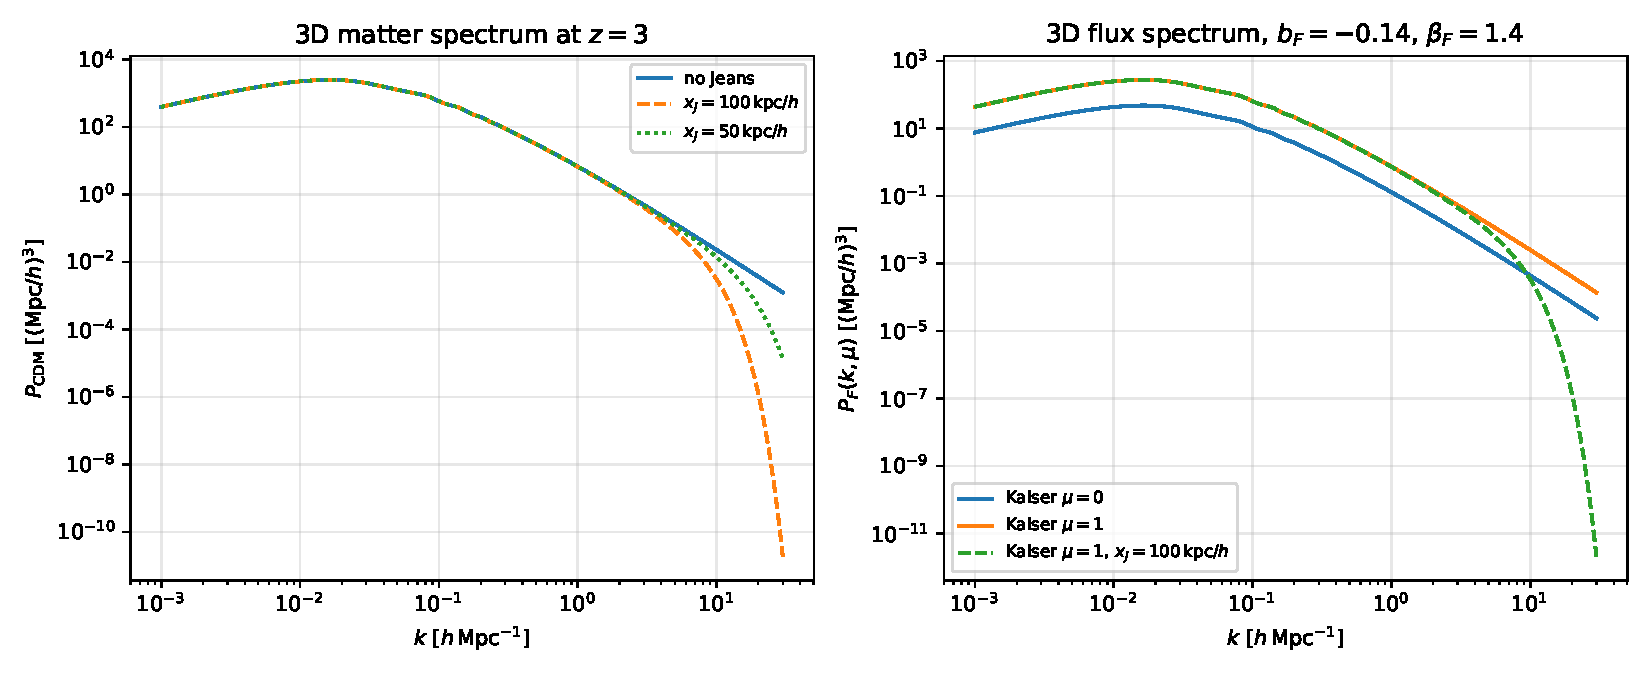
\includegraphics[width=\textwidth]{09_3d_power_spectrum.pdf}
\caption{Left: linear matter spectrum at $z=3$ with no Jeans factor and with $x_J=100$ and $50\,\mathrm{kpc}/h$.
Right: Kaiser formula \eqref{eq:kaiser} at $\mu=0$ and $\mu=1$, and the $\mu=1$ curve after the $100\,\mathrm{kpc}/h$ cutoff.
These panels evaluate the analytic expressions; they are not a measurement in a volume.}
\label{fig:jeans3d}
\end{figure}

\section{Gaussian density and lognormal density}
\label{sec:density}

Equation~\eqref{eq:lognormal} was already the density used for the optical depth in Part~I.
Figure~\ref{fig:gauss-logn} compares the one-dimensional power of $\delta_G$ with that of $\Delta-1$, on the same lines, for the three values of $x_J$.
The lines are shorter than the Part~I comparison figure, so that the Nyquist mode lies past the cutoff: length $L=40\,\mathrm{Mpc}/h$, $N=1024$ pixels, and $512$ lines, drawn with random seed $7$.
The pixel size is $L/N=0.0391\,\mathrm{Mpc}/h$, and the Nyquist wavenumber is $\pi N/L\approx 80.4\,h\,\mathrm{Mpc}^{-1}$.
The matter table used for the projection extends from $10^{-3}$ to $120\,h\,\mathrm{Mpc}^{-1}$.

\begin{figure}[htbp]
\centering
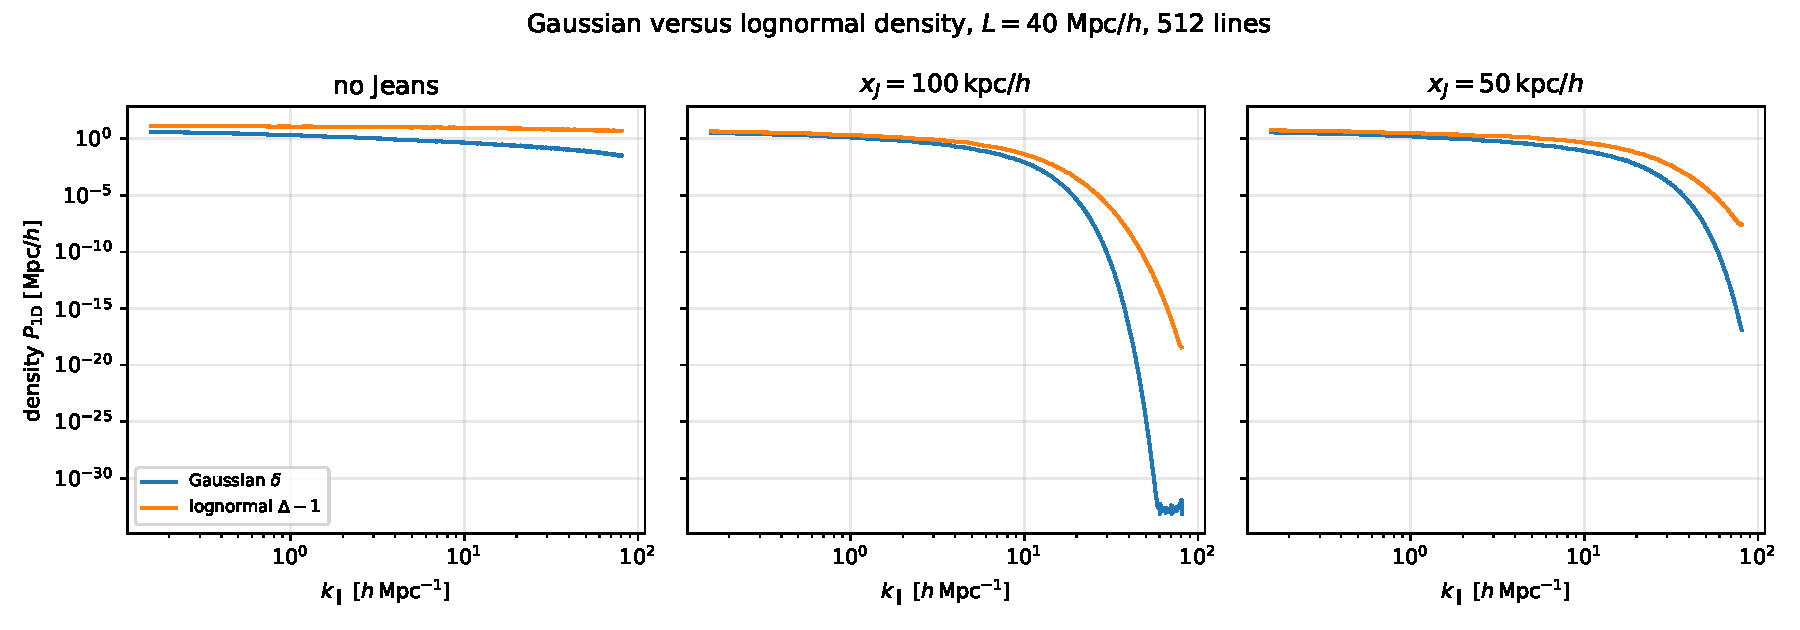
\includegraphics[width=\textwidth]{10_gaussian_vs_lognormal.pdf}
\caption{One-dimensional power of the Gaussian contrast $\delta_G$ and of the lognormal field $\Delta-1$, for $x_J=0$, $100$, and $50\,\mathrm{kpc}/h$.
Lines have length $40\,\mathrm{Mpc}/h$ and $1024$ pixels.}
\label{fig:gauss-logn}
\end{figure}

On these lines the variances and the fraction of Gaussian pixels with $1+\delta_G\le 0$ are
\begin{center}
\small
\begin{tabular}{@{}lccc@{}}
\toprule
$x_J$ & $\mathrm{Var}(\delta_G)$ & $\mathrm{Var}(\Delta)$ & fraction with $1+\delta_G\le 0$ \\
\midrule
$0$ & $6.06$ & $175$ & $0.34$ \\
$0.10\,\mathrm{Mpc}/h$ & $1.28$ & $2.42$ & $0.19$ \\
$0.05\,\mathrm{Mpc}/h$ & $1.99$ & $5.57$ & $0.24$ \\
\bottomrule
\end{tabular}
\end{center}
With the cutoff omitted, a Gaussian field $1+\delta_G$ takes negative values on a third of the pixels and cannot be used as the argument of $\Delta^{\beta}$ in Eq.~\eqref{eq:fgpa}.
The optical depth continues to be evaluated on the lognormal density, which is positive by construction.
At $100\,\mathrm{kpc}/h$ the lognormal variance has fallen to $2.4$, the regime in which the map may be described as weakly nonlinear.
At $50\,\mathrm{kpc}/h$ the variance rises again, because that length suppresses a smaller range of $k$.
In all three panels the lognormal spectrum lies above the Gaussian spectrum at high $k_\parallel$: the exponential in Eq.~\eqref{eq:lognormal} regenerates small-scale power after the cutoff has removed it from $\delta_G$.

\section{Flux power on the smoothed spectrum}
\label{sec:flux}

Figure~\ref{fig:flux-jeans} repeats the same line geometry and the same three values of $x_J$, with random seed $11$.
The left panel is the integral \eqref{eq:p1d} applied to Eq.~\eqref{eq:kaiser}, with $P_\mathrm{CDM}$ replaced by the screened spectrum.
The right panel is the periodogram of $\delta_F=F/\langle F\rangle-1$ after Eq.~\eqref{eq:fgpa}, with $A$ solved for $\langle F\rangle=0.80$.
Modes are retained where $10^{-3}<k_\parallel$ in $\mathrm{s\,km}^{-1}$ and the comoving wavenumber is below $20\,h\,\mathrm{Mpc}^{-1}$ (about $0.18\,\mathrm{s\,km}^{-1}$ at $z=3$).

\begin{figure}[htbp]
\centering
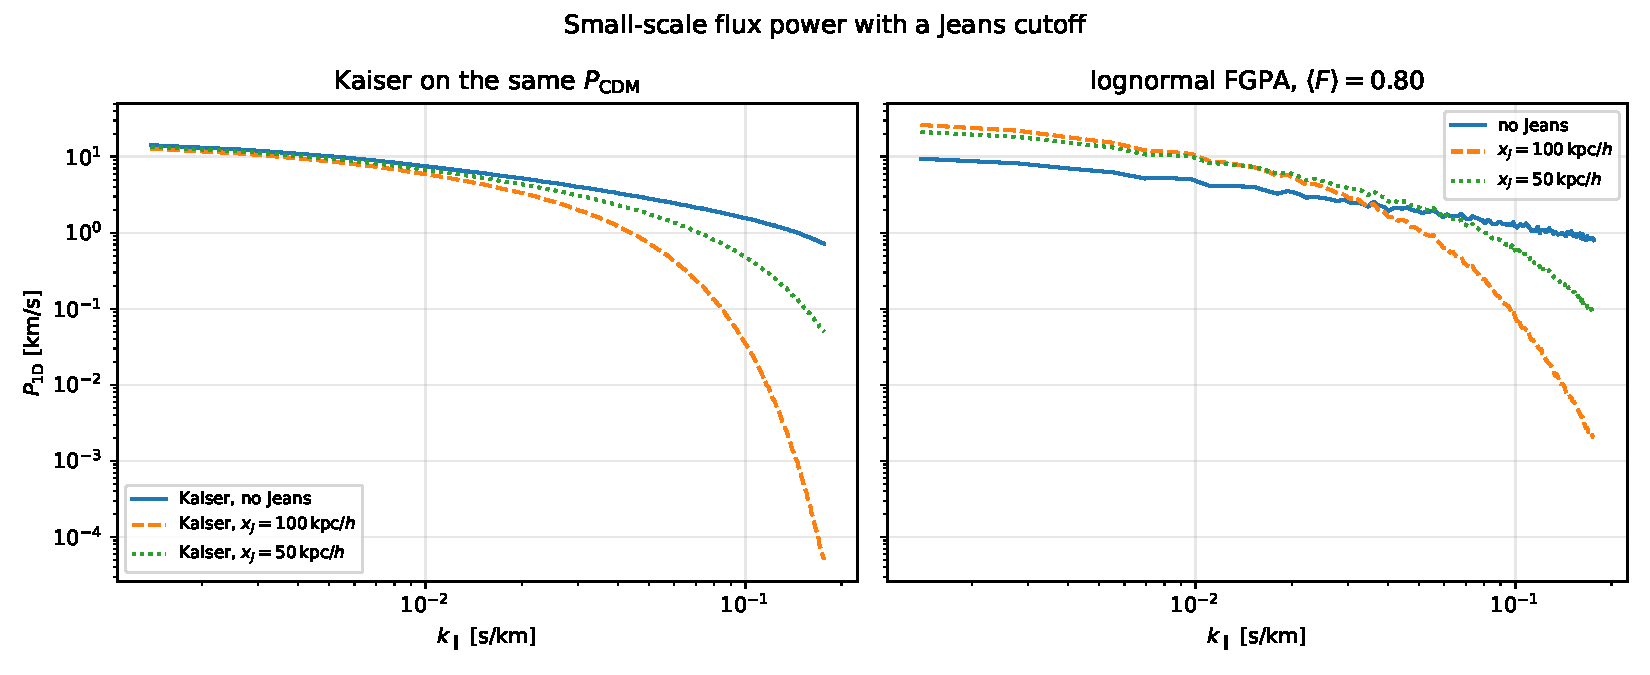
\includegraphics[width=\textwidth]{11_flux_jeans_scales.pdf}
\caption{Flux power at $z=3$ on the Jeans-smoothed spectrum.
Left: Kaiser integral.
Right: optical-depth sightlines with $\langle F\rangle=0.80$.
Below about $0.01\,\mathrm{s\,km}^{-1}$ the three curves overlie in each panel; above that, $100\,\mathrm{kpc}/h$ falls first.}
\label{fig:flux-jeans}
\end{figure}

Below about $0.01\,\mathrm{s\,km}^{-1}$ the three Kaiser curves overlie, and so do the three sightline curves.
Above that wavenumber the $100\,\mathrm{kpc}/h$ spectrum falls first in both panels.
The sightline spectra fall less steeply than the Kaiser spectra, which is the regeneration of small-scale power already seen in Sec.~\ref{sec:density}, now passed through $F=e^{-\tau}$.
The fitted amplitudes and the lognormal variances are $A=2.41$ and $\mathrm{Var}(\Delta)=115$ with no cutoff, $A=0.256$ and $\mathrm{Var}(\Delta)=2.59$ at $100\,\mathrm{kpc}/h$, and $A=0.327$ and $\mathrm{Var}(\Delta)=5.93$ at $50\,\mathrm{kpc}/h$.
The mean transmission is $0.800$ in each case.
These values of $A$ differ from the $A=0.485$ of the Part~I figure because that figure uses $L=200\,\mathrm{Mpc}/h$ and $N=512$, whose Nyquist mode is only about $8\,h\,\mathrm{Mpc}^{-1}$.
The short lines resolve the small-scale power that Eq.~\eqref{eq:jeans} is intended to remove, and the amplitude required to keep $\langle F\rangle=0.80$ changes accordingly.

\section{Sampling noise of the sightline spectrum}
\label{sec:noise}

The Part~I comparison of the two flux spectra averaged $256$ lines of length $200\,\mathrm{Mpc}/h$ with $512$ pixels.
Figure~\ref{fig:noise} repeats that geometry on a single draw of $10\,000$ lines from the unsmoothed spectrum, with seed $7$.
The optical depth is solved once on the full ensemble, giving $A=0.502$ and a mean transmission of $0.800$.
Spectra are then measured on the first $256$, $1024$, and $4096$ lines, and on all $10\,000$ lines.
For each subset the flux contrast uses the mean transmission of that subset.

\begin{figure}[htbp]
\centering
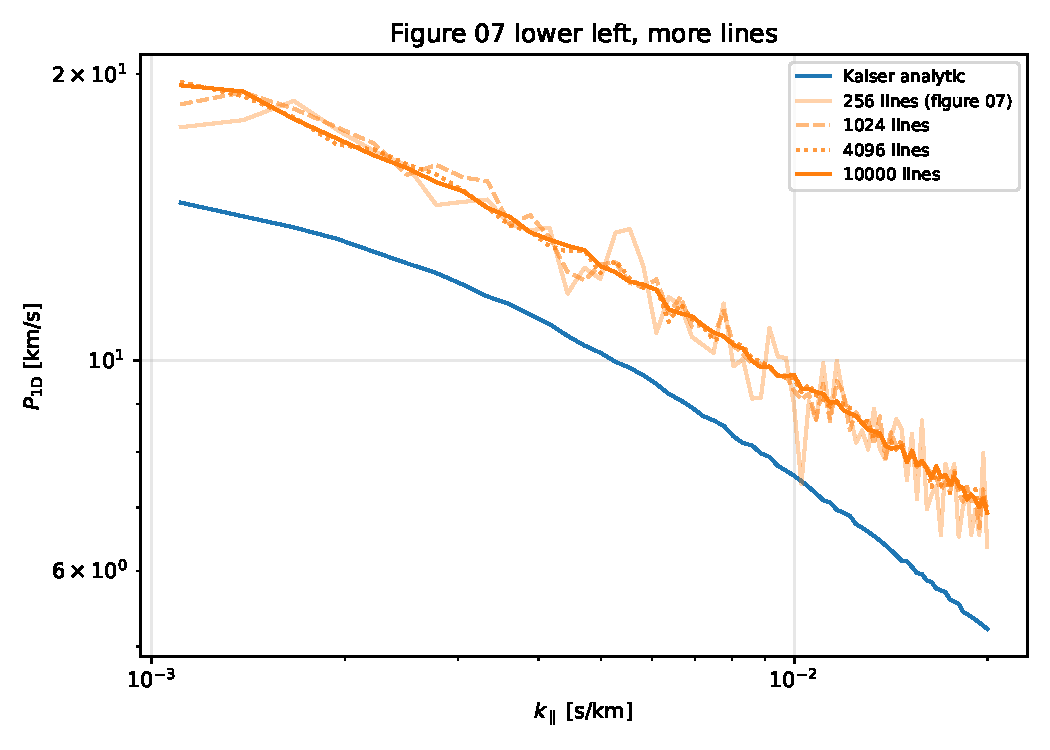
\includegraphics[width=0.82\textwidth]{12_skewer_noise.pdf}
\caption{Sightline flux power for subsets of one $10\,000$-line draw at $z=3$, compared with the Kaiser curve.
The scatter falls as the ensemble grows; the vertical offset from Kaiser remains at $10\,000$ lines.}
\label{fig:noise}
\end{figure}

Over $10^{-3}<k_\parallel<0.02\,\mathrm{s\,km}^{-1}$, the root-mean-square fractional difference from the $10\,000$-line spectrum is $0.067$ for $256$ lines, $0.030$ for $1024$ lines, and $0.012$ for $4096$ lines.
The ratio of the $256$-line and $1024$-line numbers is $2.28$, against $\sqrt{4}=2$ for a scatter that scales as $N_\mathrm{lines}^{-1/2}$.
The ratio of the $256$-line and $4096$-line numbers is $5.47$, against $\sqrt{16}=4$.
A split of the same draw into $39$ contiguous blocks of $256$ lines has a median fractional scatter of $0.061$ about the mean of the blocks.

An ensemble of $500$ lines in place of $256$ would reduce this scatter by $\sqrt{256/500}\approx 0.72$.
The vertical offset between the sightline spectrum and the Kaiser spectrum remains at $10\,000$ lines.
That offset is the difference between a mean transmission of $0.80$ in real space and the fixed bias of Eq.~\eqref{eq:kaiser}; it is not sample variance.

\section{Flux spectra at $z=5$}
\label{sec:z5}

At $z=5$ in the fiducial cosmology,
\begin{equation}
\frac{\mathrm{d}v}{\mathrm{d}\chi}
=
\frac{H(z)}{(1+z)\,h}
=
137\,\mathrm{km\,s}^{-1}
\text{ per }\mathrm{Mpc}/h,
\end{equation}
so $k_\parallel=0.2\,\mathrm{s\,km}^{-1}$ corresponds to $27.4\,h\,\mathrm{Mpc}^{-1}$.
Figure~\ref{fig:z5} uses lines of length $L=40\,\mathrm{Mpc}/h$ with $N=512$ pixels and $256$ lines, so the Nyquist mode is $\pi N/L=40.2\,h\,\mathrm{Mpc}^{-1}$, past the requested scale.
The matter table runs from $10^{-3}$ to $80\,h\,\mathrm{Mpc}^{-1}$.
The Kaiser integral is carried to that same upper limit, rather than to the $30\,h\,\mathrm{Mpc}^{-1}$ cutoff of Part~I, so that $27\,h\,\mathrm{Mpc}^{-1}$ does not sit on the edge of the quadrature.
The three values of $x_J$ are again $0$, $0.10$, and $0.05\,\mathrm{Mpc}/h$.

The mean transmission is taken from the power-law fit of Faucher-Gigu\`ere et al., with metals left in the forest \citep{Faucher-Giguere:2007ab},
\begin{equation}
\label{eq:taueff}
\tau_{\mathrm{eff}}(z)=0.0018\,(1+z)^{3.92},
\qquad
\langle F\rangle=e^{-\tau_{\mathrm{eff}}}.
\end{equation}
That fit was measured on $2\le z\le 4.2$.
At $z=5$ it is an extrapolation: $\tau_{\mathrm{eff}}=2.02$ and $\langle F\rangle=0.132$.
It replaces the value $0.80$ used at $z=3$; a transmission of $0.80$ would leave the $z=5$ forest almost transparent.
The temperature--density index remains $\gamma=1.5$.

\begin{figure}[htbp]
\centering
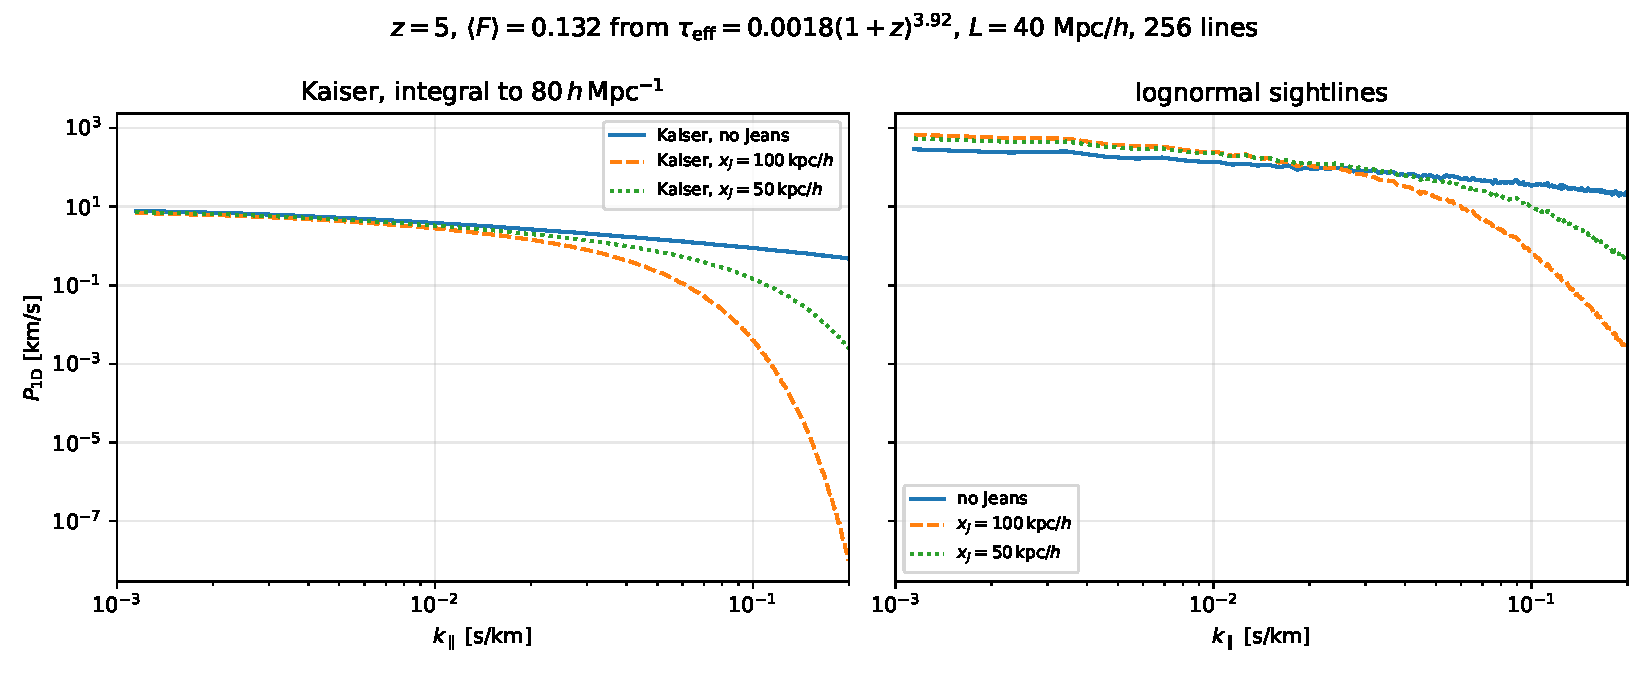
\includegraphics[width=\textwidth]{13_z5_smallscale_flux.pdf}
\caption{Flux power at $z=5$ out to $0.2\,\mathrm{s\,km}^{-1}$.
Left: Kaiser integral.
Right: optical-depth sightlines with $\langle F\rangle=0.132$ from the extrapolated Faucher-Gigu\`ere fit.
The three Jeans lengths are $0$, $100$, and $50\,\mathrm{kpc}/h$.}
\label{fig:z5}
\end{figure}

On these lines the Gaussian variance, the lognormal variance, and the fitted amplitude are $2.21$, $6.72$, and $A=74.1$ with no cutoff; $0.582$, $0.780$, and $A=6.25$ at $100\,\mathrm{kpc}/h$; and $0.903$, $1.41$, and $A=10.7$ at $50\,\mathrm{kpc}/h$.
The mean transmission is $0.132$ in each case.
With the $100\,\mathrm{kpc}/h$ cutoff the density is weakly nonlinear.
Without it, $A$ is large because the target transmission is low and the lines still resolve small-scale power.

In the Kaiser panel the three curves overlie below about $0.01\,\mathrm{s\,km}^{-1}$, and $100\,\mathrm{kpc}/h$ falls first above that.
The sightline panel has the same ordering at high $k_\parallel$ and a much larger amplitude at every plotted $k_\parallel$.
The sightline amplitude is fixed by $\langle F\rangle=0.132$; the Kaiser amplitude is still fixed by $b_F=-0.14$.
Those two normalisations are different conditions, and at this transmission the difference is a factor of several tens in $P_{1\mathrm{D}}$.

\section{Three-dimensional flux power}
\label{sec:box}

\subsection{Geometry and velocity}

Figure~\ref{fig:box} is one periodic cube of side $L=40\,\mathrm{Mpc}/h$ and $128^{3}$ cells, at $z=3$, with the Jeans length $x_J=0.10\,\mathrm{Mpc}/h$.
The fundamental mode is $2\pi/L=0.157\,h\,\mathrm{Mpc}^{-1}$ and the Nyquist mode is $\pi N/L=10.1\,h\,\mathrm{Mpc}^{-1}$.
Each Fourier amplitude is set to the root-mean-square of $P(k)$, with a random phase, which is the same choice Arinyo-i-Prats et al.\ made for the initial conditions of their hydrodynamic runs \citep{Arinyo-i-Prats:2015vqa}.
The Gaussian variance in the cube is $1.38$ and the lognormal variance is $2.85$.

The line-of-sight peculiar velocity is the linear continuity field of that Gaussian density.
If $\delta(\mathbf{k})$ is the Fourier transform of the contrast, the comoving shift is
\begin{equation}
\label{eq:disp}
\psi_\parallel(\mathbf{k})
=
\mathrm{i}\,f\,\frac{k_\parallel}{k^{2}}\,\delta(\mathbf{k}),
\end{equation}
with the logarithmic growth rate $f=\mathrm{d}\ln D/\mathrm{d}\ln a$ taken from the growth function of Part~I; at $z=3$ one has $f=0.982$.
The real-space field $\psi_\parallel$ has an rms of $0.98\,\mathrm{Mpc}/h$, about three cells.
Optical depth is deposited in redshift space by a periodic cloud-in-cell shift of $\tau$ along one axis, and $A$ is solved afterwards so that $\langle F\rangle$ equals the target.
The target mean transmission is $0.696$, the value used at $z=3$ in the hydrodynamic comparison of Arinyo-i-Prats et al., rather than the $0.80$ of Part~I.
The fitted amplitude is $A=0.569$ in real space and $A=0.920$ after the shift; both give $\langle F\rangle=0.696$.

\subsection{Published nonlinear model}

The published model compared with this cube is \citep{Arinyo-i-Prats:2015vqa}
\begin{equation}
\label{eq:arinyo}
P_F(k,\mu)
=
b_{F\delta}^{2}\,(1+\beta\mu^{2})^{2}\,P_L(k)\,D_1(k,\mu),
\end{equation}
with the nonlinear factor (their equation~3.6, with $q_2=0$)
\begin{equation}
\label{eq:d1}
D_1(k,\mu)
=
\exp\left\{
q_1\Delta^{2}(k)
\left[1-\left(\frac{k}{k_v}\right)^{a_v}\mu^{b_v}\right]
-
\left(\frac{k}{k_p}\right)^{2}
\right\},
\qquad
\Delta^{2}(k)=\frac{k^{3}P_L(k)}{2\pi^{2}}.
\end{equation}
$P_L$ is the linear Eisenstein--Hu spectrum of this calculation, without an additional Jeans factor: $D_1$ already contains a pressure scale $k_p$.
The numbers are the fiducial simulation at $z=3$ in their Tables~2 and~3, and they are not refitted:
\begin{equation}
\begin{aligned}
q_1 &= 0.648, &
k_p &= 13.1\,h\,\mathrm{Mpc}^{-1}, &
k_v^{a_v} &= 1.007, \\
a_v &= 0.627, &
b_v &= 1.66, &
\beta &= 1.205.
\end{aligned}
\end{equation}
Their density bias is quoted for the effective optical depth, $b_{\tau\delta}=0.5546$.
The transmission bias follows their relation
\begin{equation}
\label{eq:btau}
b_{F\delta}=b_{\tau\delta}\ln\langle F\rangle=-0.201
\quad\text{at}\quad
\langle F\rangle=0.696.
\end{equation}
Their cosmological parameters and thermal history are not those of this calculation.
The overlay is the published formula evaluated on this $P_L$.

\subsection{Estimator check and results}

A field constructed as $b_F(1+\beta_F\mu^{2})\delta(\mathbf{k})$, with the Part~I values $b_F=-0.14$ and $\beta_F=1.4$, recovers Eq.~\eqref{eq:kaiser} mode by mode.
The largest fractional residual on the nonzero modes of this cube is $9\times 10^{-14}$.
The estimator applied to the optical-depth cube is therefore the same one that recovers the analytic Kaiser field.

Figure~\ref{fig:box} shows two bins, $\mu<0.25$ and $\mu>0.75$.
The Kaiser curve uses $b_F=-0.14$ and the screened matter spectrum.
The Arinyo-i-Prats curve uses Eq.~\eqref{eq:arinyo}.
The other two curves are the lognormal flux in real space and after the linear shift \eqref{eq:disp}.
At $k=1.16\,h\,\mathrm{Mpc}^{-1}$ the ratios to the Part~I Kaiser curve are $6.29$ (real space) and $5.41$ (redshift space) for $\mu<0.25$, and $1.64$ and $2.44$ for $\mu>0.75$.
The same redshift-space measurement divided by Eq.~\eqref{eq:arinyo} is $2.05$ and $1.31$ in those two bins.
The redshift-space cube lies above the real-space cube for $\mu>0.75$ and below it for $\mu<0.25$, which is the sense of the Kaiser factor.
Its slope follows the published formula.
Its amplitude does not: the lognormal map at $\langle F\rangle=0.696$, on a matter spectrum that already carries $x_J=0.10\,\mathrm{Mpc}/h$, is a different model from the hydrodynamic calibration, and from the fixed bias $b_F=-0.14$.

\begin{figure}[htbp]
\centering
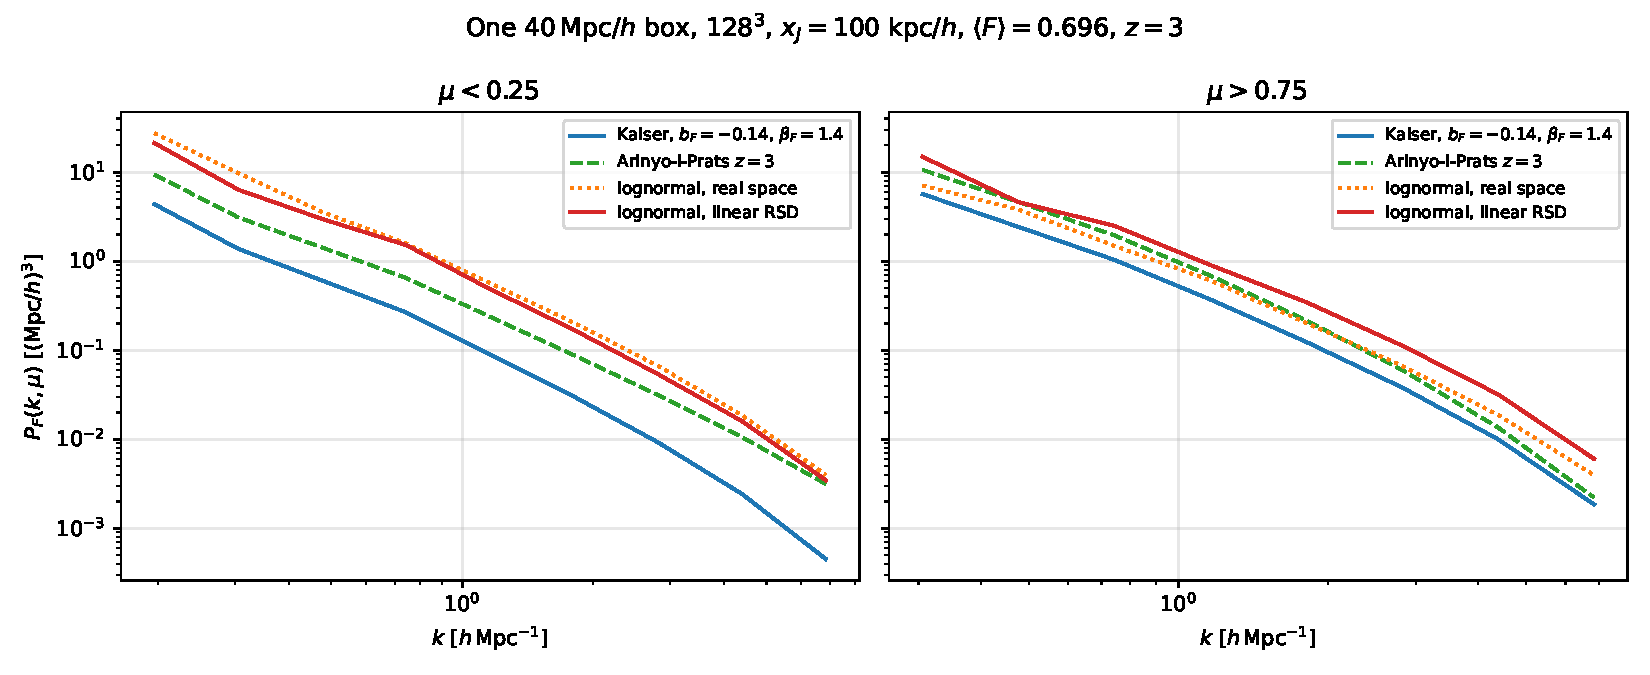
\includegraphics[width=\textwidth]{14_p3d_kmu.pdf}
\caption{Measured $P_F(k,\mu)$ in one $40\,\mathrm{Mpc}/h$, $128^{3}$ cube at $z=3$ with $x_J=100\,\mathrm{kpc}/h$ and $\langle F\rangle=0.696$, for $\mu<0.25$ (left) and $\mu>0.75$ (right).
Solid: Part~I Kaiser formula on the screened spectrum.
Dashed: Arinyo-i-Prats formula at the published $z=3$ parameters.
Dotted and solid red: lognormal flux in real space and after the linear line-of-sight shift.}
\label{fig:box}
\end{figure}

% Post-meeting full-physics upgrade (figures 15--16). Comment out if compiling without those PDFs.
% Overleaf drop-in note: upgrades after the Tuesday meeting (Kier / Vera / Simeon).
% Paste after the ``Three-dimensional flux power'' section of part2.tex, or
% % Overleaf drop-in note: upgrades after the Tuesday meeting (Kier / Vera / Simeon).
% Paste after the ``Three-dimensional flux power'' section of part2.tex, or
% % Overleaf drop-in note: upgrades after the Tuesday meeting (Kier / Vera / Simeon).
% Paste after the ``Three-dimensional flux power'' section of part2.tex, or
% \input{update_post_meeting} from the main file. Figures live in plots/.
%
% Companion script: make_full_physics_plots.py
% Figures: 15_full_physics_p1d_p3d.pdf, 16_full_physics_param_vary.pdf

\section{Post-meeting upgrade: full physics in one realisation}
\label{sec:fullphysics}

\subsection{Motivation}

The Tuesday discussion asked for $P_{1\mathrm{D}}(k_\parallel)$ and $P_F(k,\mu)$ measured from sightlines that include the same physics: lognormal density, Jeans smoothing, thermal broadening, FGPA optical depth, and peculiar velocities.
Section~\ref{sec:box} already had Jeans, lognormal, FGPA, and linear redshift-space distortions in the cube, but thermal broadening was off, and $P_{1\mathrm{D}}$ was not taken from that same volume.
The 1D FGPA sightlines of Part~I remained in real space.

\subsection{What changed relative to Figure~\ref{fig:box}}

\begin{center}
\small
\begin{tabular}{@{}lll@{}}
\toprule
Ingredient & Figure~\ref{fig:box} (meeting) & This update \\
\midrule
Jeans $x_J$ on $P_\mathrm{CDM}$ & $100\,\mathrm{kpc}/h$ & same \\
Lognormal $\Delta$ + FGPA $\tau=A\Delta^{\beta}$ & yes & same \\
Linear peculiar velocities (CIC on $\tau$) & yes & same \\
Thermal Gaussian on $\tau$ (after the shift) & off & on ($\sigma_v=10\,\mathrm{km\,s}^{-1}$ fiducial) \\
$\langle F\rangle$ & $0.696$ & same \\
$P_F(k,\mu)$ from the cube & yes & yes \\
$P_{1\mathrm{D}}$ from the same LOS skewers & no & yes \\
Parameter variations & no & $A_s$, $n_s$, $x_J$, $\sigma_{v,\mathrm{th}}$ \\
\bottomrule
\end{tabular}
\end{center}

The processing order in the cube is now
\begin{equation}
\delta_G
\;\to\;
\Delta=\mathrm{e}^{\delta_G-\sigma_G^{2}/2}
\;\to\;
\tau_\mathrm{unit}=\Delta^{\beta}
\;\to\;
\text{CIC shift by }\psi_\parallel
\;\to\;
\text{thermal smooth along the LOS}
\;\to\;
\text{solve }A\text{ so }\langle\mathrm{e}^{-A\tau}\rangle=\langle F\rangle.
\end{equation}
The thermal width is specified in $\mathrm{km\,s}^{-1}$ and converted to comoving $\mathrm{Mpc}/h$ with $H(z)/((1+z)h)$, then to pixels with the cell size $L/N$.
At $z=3$, $\sigma_v=10\,\mathrm{km\,s}^{-1}$ corresponds to $\sigma_x\approx 0.088\,\mathrm{Mpc}/h$ ($\sim 0.3$ cells on the $40\,\mathrm{Mpc}/h$, $128^{3}$ grid).

Every transverse cell provides one line-of-sight skewer.
$P_{1\mathrm{D}}$ is the ensemble periodogram of those $N^{2}$ flux-contrast skewers; $P_F(k,\mu)$ is the same 3D contrast binned in $k$ and $\mu$.
Both therefore share one seed, one Jeans length, one thermal width, and one fitted $A$.

\subsection{Fiducial measurement}

Figure~\ref{fig:fullphysics} uses the same geometry as Figure~\ref{fig:box}: $L=40\,\mathrm{Mpc}/h$, $N=128$, $z=3$, $x_J=100\,\mathrm{kpc}/h$, $\langle F\rangle=0.696$, linear growth rate $f\approx 0.982$.
The left panel is $P_{1\mathrm{D}}(k_\parallel)$ from the box skewers, with the analytic Kaiser $P_{1\mathrm{D}}$ on the Jeans-smoothed spectrum for reference.
The middle and right panels are $P_F(k,\mu)$ for $\mu<0.25$ and $\mu>0.75$, with the Part~I Kaiser formula and the published Arinyo-i-Prats $z=3$ formula overlaid (still not refitted).

\begin{figure}[htbp]
\centering
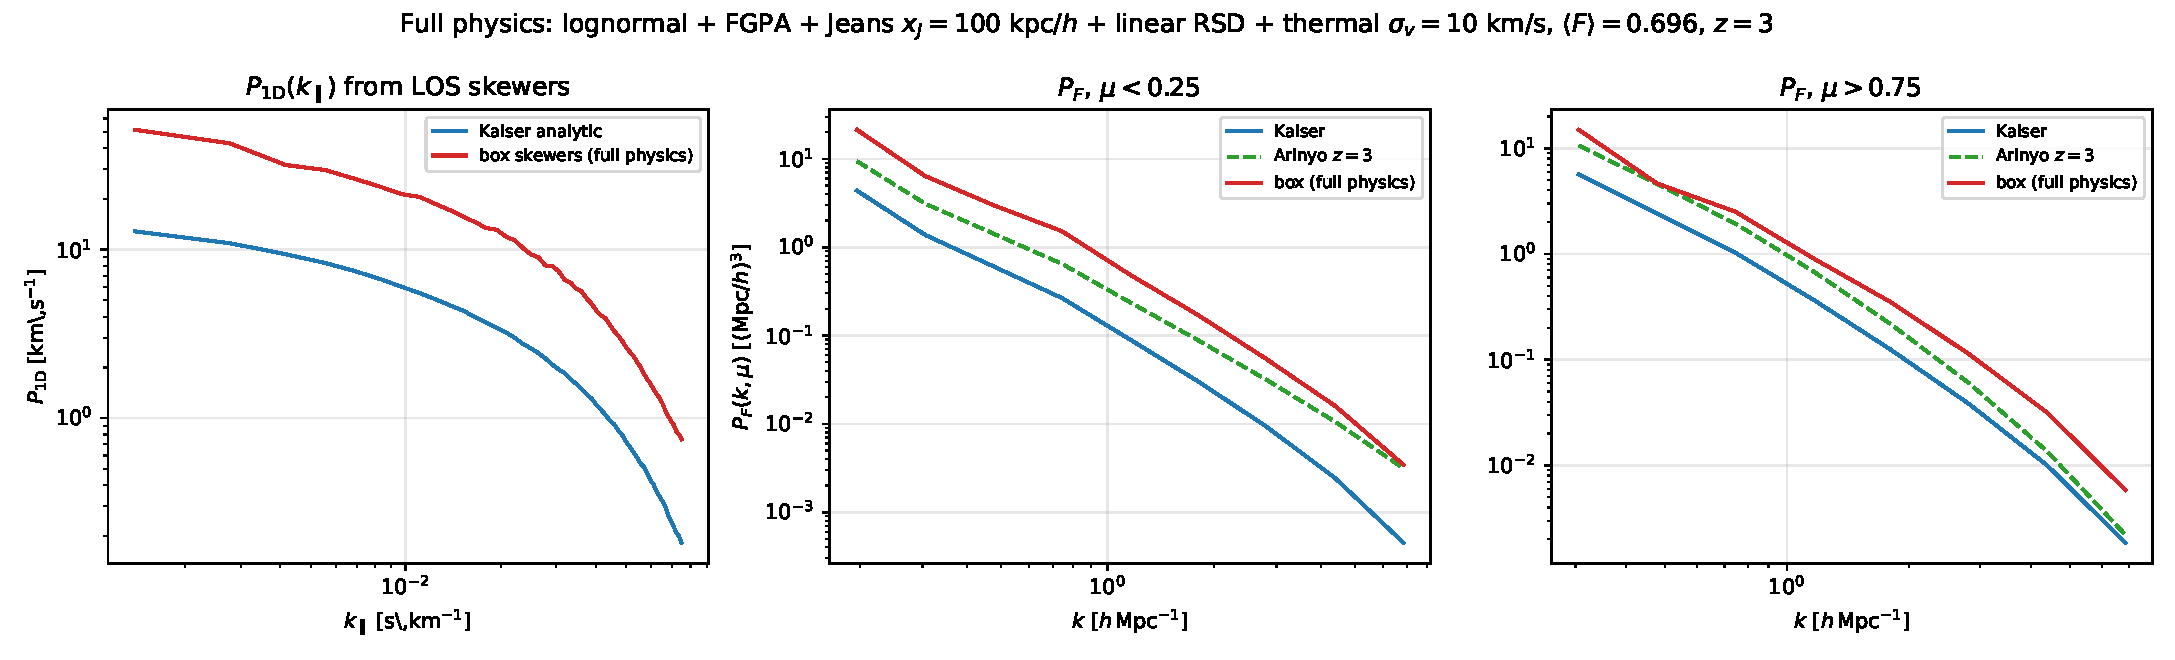
\includegraphics[width=\textwidth]{15_full_physics_p1d_p3d.pdf}
\caption{Full-physics measurement from one cube: lognormal FGPA, Jeans $x_J=100\,\mathrm{kpc}/h$, linear RSD, and thermal $\sigma_v=10\,\mathrm{km\,s}^{-1}$, at $\langle F\rangle=0.696$ and $z=3$.
Left: $P_{1\mathrm{D}}$ from all LOS skewers versus the analytic Kaiser projection.
Middle / right: $P_F(k,\mu)$ for mostly transverse and mostly parallel modes, with Kaiser and Arinyo-i-Prats overlays.}
\label{fig:fullphysics}
\end{figure}

As in Section~\ref{sec:box}, the lognormal amplitude lies above the fixed-bias Kaiser curve and above the published Arinyo formula; the slope remains closer to Arinyo than the amplitude does.
The main limits are unchanged: one small box, linear velocities only, and no refit of the Arinyo parameters.
Thermal broadening is now on, but the fiducial $10\,\mathrm{km\,s}^{-1}$ is only a fraction of a cell, so its effect is mild until $\sigma_v$ is raised (Figure~\ref{fig:paramvary}).

\subsection{Varying parameters}

Figure~\ref{fig:paramvary} repeats the full-physics cube while changing one parameter at a time, always measuring $P_{1\mathrm{D}}$ from the LOS skewers.
The four panels are $A_s$, $n_s$, the Jeans filter $\lambda_\mathrm{filter}\equiv x_J$, and the thermal width $\sigma_{v,\mathrm{th}}$.
The same random seed is kept so that changes in shape are not dominated by a new phase draw.

\begin{figure}[htbp]
\centering
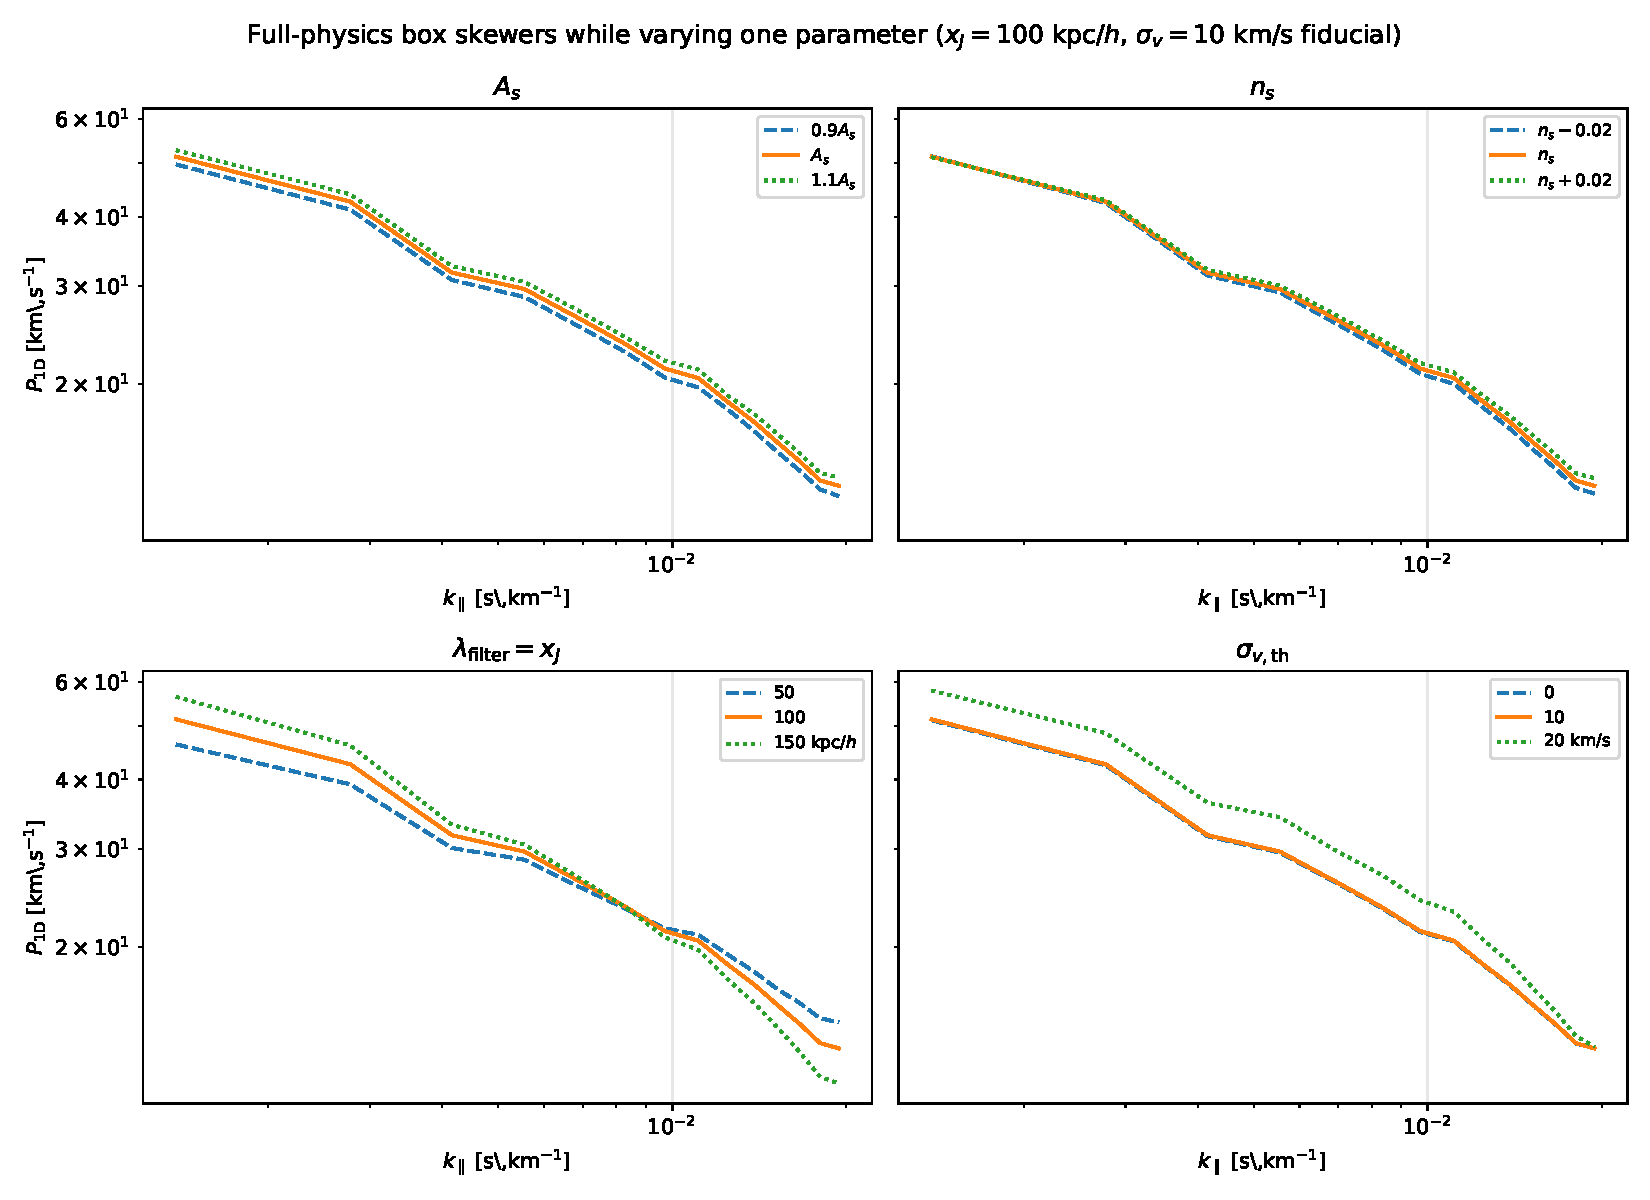
\includegraphics[width=\textwidth]{16_full_physics_param_vary.pdf}
\caption{Response of the full-physics box $P_{1\mathrm{D}}$ to one-parameter variations around the fiducial model of Figure~\ref{fig:fullphysics}.}
\label{fig:paramvary}
\end{figure}

\subsection{Code entry points}

\begin{center}
\small
\begin{tabular}{@{}p{0.42\textwidth}p{0.52\textwidth}@{}}
\toprule
Operation & Where \\
\midrule
Thermal width after RSD in the cube &
\texttt{fgpa\_flux\_box(..., thermal\_sigma\_mpch=...)} in \path{p1d/box3d.py} \\
Full-physics $P_{1\mathrm{D}}$ + $P_F(k,\mu)$ + variations &
\path{make\_full\_physics\_plots.py} \\
CLI knobs &
\texttt{--As}, \texttt{--ns}, \texttt{--lambda-filter}, \texttt{--thermal-kms}, \texttt{--mean-flux} \\
JAX twin of the pipeline (for later Fisher derivatives) &
\path{p1d\_jax/} (NumPy \path{p1d/} unchanged) \\
\bottomrule
\end{tabular}
\end{center}

Regenerate the figures with
\begin{verbatim}
python make_full_physics_plots.py
python make_full_physics_plots.py --As 2.3e-9 --ns 0.96 \
    --lambda-filter 0.1 --thermal-kms 10
\end{verbatim}
 from the main file. Figures live in plots/.
%
% Companion script: make_full_physics_plots.py
% Figures: 15_full_physics_p1d_p3d.pdf, 16_full_physics_param_vary.pdf

\section{Post-meeting upgrade: full physics in one realisation}
\label{sec:fullphysics}

\subsection{Motivation}

The Tuesday discussion asked for $P_{1\mathrm{D}}(k_\parallel)$ and $P_F(k,\mu)$ measured from sightlines that include the same physics: lognormal density, Jeans smoothing, thermal broadening, FGPA optical depth, and peculiar velocities.
Section~\ref{sec:box} already had Jeans, lognormal, FGPA, and linear redshift-space distortions in the cube, but thermal broadening was off, and $P_{1\mathrm{D}}$ was not taken from that same volume.
The 1D FGPA sightlines of Part~I remained in real space.

\subsection{What changed relative to Figure~\ref{fig:box}}

\begin{center}
\small
\begin{tabular}{@{}lll@{}}
\toprule
Ingredient & Figure~\ref{fig:box} (meeting) & This update \\
\midrule
Jeans $x_J$ on $P_\mathrm{CDM}$ & $100\,\mathrm{kpc}/h$ & same \\
Lognormal $\Delta$ + FGPA $\tau=A\Delta^{\beta}$ & yes & same \\
Linear peculiar velocities (CIC on $\tau$) & yes & same \\
Thermal Gaussian on $\tau$ (after the shift) & off & on ($\sigma_v=10\,\mathrm{km\,s}^{-1}$ fiducial) \\
$\langle F\rangle$ & $0.696$ & same \\
$P_F(k,\mu)$ from the cube & yes & yes \\
$P_{1\mathrm{D}}$ from the same LOS skewers & no & yes \\
Parameter variations & no & $A_s$, $n_s$, $x_J$, $\sigma_{v,\mathrm{th}}$ \\
\bottomrule
\end{tabular}
\end{center}

The processing order in the cube is now
\begin{equation}
\delta_G
\;\to\;
\Delta=\mathrm{e}^{\delta_G-\sigma_G^{2}/2}
\;\to\;
\tau_\mathrm{unit}=\Delta^{\beta}
\;\to\;
\text{CIC shift by }\psi_\parallel
\;\to\;
\text{thermal smooth along the LOS}
\;\to\;
\text{solve }A\text{ so }\langle\mathrm{e}^{-A\tau}\rangle=\langle F\rangle.
\end{equation}
The thermal width is specified in $\mathrm{km\,s}^{-1}$ and converted to comoving $\mathrm{Mpc}/h$ with $H(z)/((1+z)h)$, then to pixels with the cell size $L/N$.
At $z=3$, $\sigma_v=10\,\mathrm{km\,s}^{-1}$ corresponds to $\sigma_x\approx 0.088\,\mathrm{Mpc}/h$ ($\sim 0.3$ cells on the $40\,\mathrm{Mpc}/h$, $128^{3}$ grid).

Every transverse cell provides one line-of-sight skewer.
$P_{1\mathrm{D}}$ is the ensemble periodogram of those $N^{2}$ flux-contrast skewers; $P_F(k,\mu)$ is the same 3D contrast binned in $k$ and $\mu$.
Both therefore share one seed, one Jeans length, one thermal width, and one fitted $A$.

\subsection{Fiducial measurement}

Figure~\ref{fig:fullphysics} uses the same geometry as Figure~\ref{fig:box}: $L=40\,\mathrm{Mpc}/h$, $N=128$, $z=3$, $x_J=100\,\mathrm{kpc}/h$, $\langle F\rangle=0.696$, linear growth rate $f\approx 0.982$.
The left panel is $P_{1\mathrm{D}}(k_\parallel)$ from the box skewers, with the analytic Kaiser $P_{1\mathrm{D}}$ on the Jeans-smoothed spectrum for reference.
The middle and right panels are $P_F(k,\mu)$ for $\mu<0.25$ and $\mu>0.75$, with the Part~I Kaiser formula and the published Arinyo-i-Prats $z=3$ formula overlaid (still not refitted).

\begin{figure}[htbp]
\centering
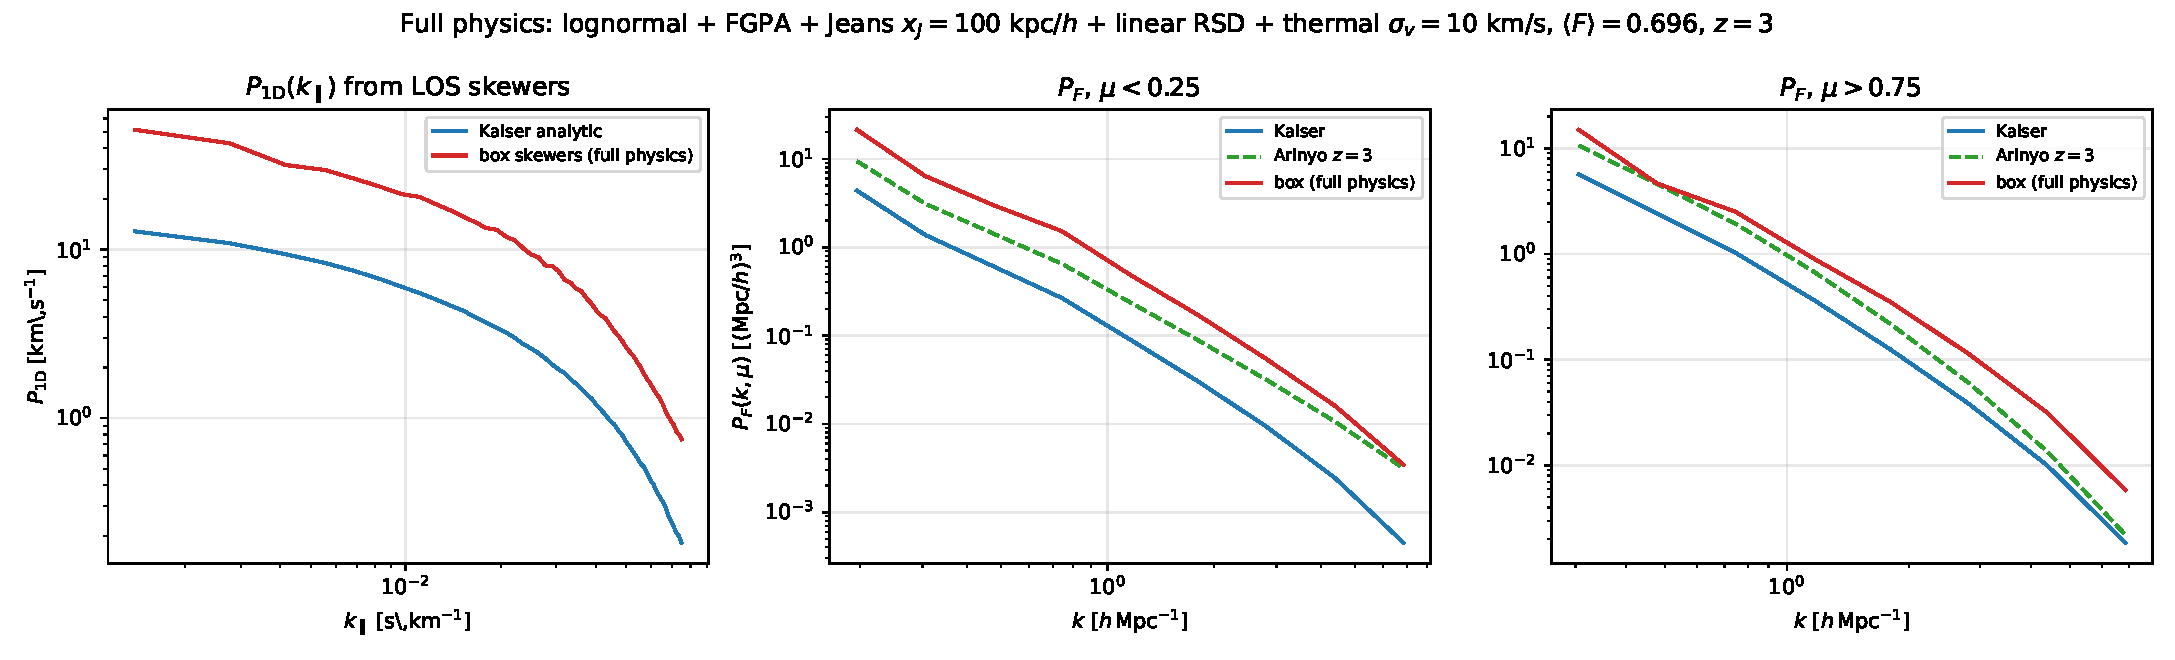
\includegraphics[width=\textwidth]{15_full_physics_p1d_p3d.pdf}
\caption{Full-physics measurement from one cube: lognormal FGPA, Jeans $x_J=100\,\mathrm{kpc}/h$, linear RSD, and thermal $\sigma_v=10\,\mathrm{km\,s}^{-1}$, at $\langle F\rangle=0.696$ and $z=3$.
Left: $P_{1\mathrm{D}}$ from all LOS skewers versus the analytic Kaiser projection.
Middle / right: $P_F(k,\mu)$ for mostly transverse and mostly parallel modes, with Kaiser and Arinyo-i-Prats overlays.}
\label{fig:fullphysics}
\end{figure}

As in Section~\ref{sec:box}, the lognormal amplitude lies above the fixed-bias Kaiser curve and above the published Arinyo formula; the slope remains closer to Arinyo than the amplitude does.
The main limits are unchanged: one small box, linear velocities only, and no refit of the Arinyo parameters.
Thermal broadening is now on, but the fiducial $10\,\mathrm{km\,s}^{-1}$ is only a fraction of a cell, so its effect is mild until $\sigma_v$ is raised (Figure~\ref{fig:paramvary}).

\subsection{Varying parameters}

Figure~\ref{fig:paramvary} repeats the full-physics cube while changing one parameter at a time, always measuring $P_{1\mathrm{D}}$ from the LOS skewers.
The four panels are $A_s$, $n_s$, the Jeans filter $\lambda_\mathrm{filter}\equiv x_J$, and the thermal width $\sigma_{v,\mathrm{th}}$.
The same random seed is kept so that changes in shape are not dominated by a new phase draw.

\begin{figure}[htbp]
\centering
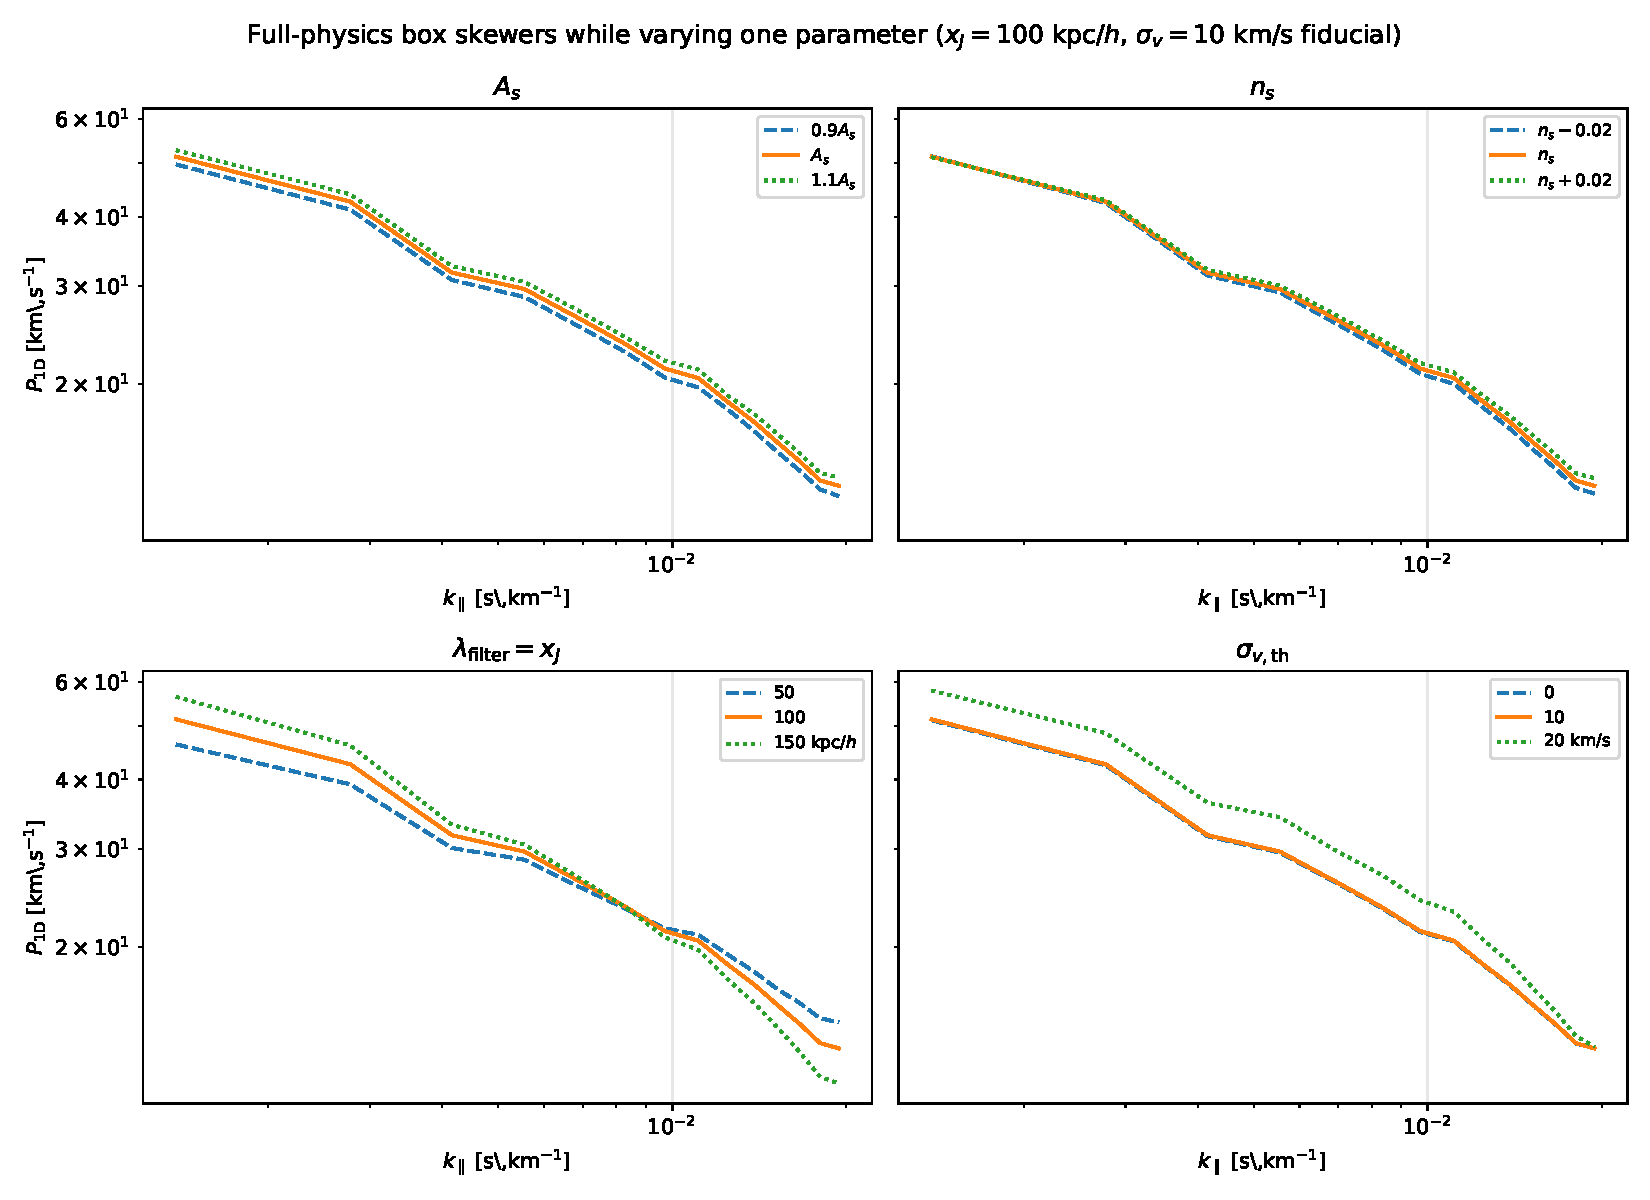
\includegraphics[width=\textwidth]{16_full_physics_param_vary.pdf}
\caption{Response of the full-physics box $P_{1\mathrm{D}}$ to one-parameter variations around the fiducial model of Figure~\ref{fig:fullphysics}.}
\label{fig:paramvary}
\end{figure}

\subsection{Code entry points}

\begin{center}
\small
\begin{tabular}{@{}p{0.42\textwidth}p{0.52\textwidth}@{}}
\toprule
Operation & Where \\
\midrule
Thermal width after RSD in the cube &
\texttt{fgpa\_flux\_box(..., thermal\_sigma\_mpch=...)} in \path{p1d/box3d.py} \\
Full-physics $P_{1\mathrm{D}}$ + $P_F(k,\mu)$ + variations &
\path{make\_full\_physics\_plots.py} \\
CLI knobs &
\texttt{--As}, \texttt{--ns}, \texttt{--lambda-filter}, \texttt{--thermal-kms}, \texttt{--mean-flux} \\
JAX twin of the pipeline (for later Fisher derivatives) &
\path{p1d\_jax/} (NumPy \path{p1d/} unchanged) \\
\bottomrule
\end{tabular}
\end{center}

Regenerate the figures with
\begin{verbatim}
python make_full_physics_plots.py
python make_full_physics_plots.py --As 2.3e-9 --ns 0.96 \
    --lambda-filter 0.1 --thermal-kms 10
\end{verbatim}
 from the main file. Figures live in plots/.
%
% Companion script: make_full_physics_plots.py
% Figures: 15_full_physics_p1d_p3d.pdf, 16_full_physics_param_vary.pdf

\section{Post-meeting upgrade: full physics in one realisation}
\label{sec:fullphysics}

\subsection{Motivation}

The Tuesday discussion asked for $P_{1\mathrm{D}}(k_\parallel)$ and $P_F(k,\mu)$ measured from sightlines that include the same physics: lognormal density, Jeans smoothing, thermal broadening, FGPA optical depth, and peculiar velocities.
Section~\ref{sec:box} already had Jeans, lognormal, FGPA, and linear redshift-space distortions in the cube, but thermal broadening was off, and $P_{1\mathrm{D}}$ was not taken from that same volume.
The 1D FGPA sightlines of Part~I remained in real space.

\subsection{What changed relative to Figure~\ref{fig:box}}

\begin{center}
\small
\begin{tabular}{@{}lll@{}}
\toprule
Ingredient & Figure~\ref{fig:box} (meeting) & This update \\
\midrule
Jeans $x_J$ on $P_\mathrm{CDM}$ & $100\,\mathrm{kpc}/h$ & same \\
Lognormal $\Delta$ + FGPA $\tau=A\Delta^{\beta}$ & yes & same \\
Linear peculiar velocities (CIC on $\tau$) & yes & same \\
Thermal Gaussian on $\tau$ (after the shift) & off & on ($\sigma_v=10\,\mathrm{km\,s}^{-1}$ fiducial) \\
$\langle F\rangle$ & $0.696$ & same \\
$P_F(k,\mu)$ from the cube & yes & yes \\
$P_{1\mathrm{D}}$ from the same LOS skewers & no & yes \\
Parameter variations & no & $A_s$, $n_s$, $x_J$, $\sigma_{v,\mathrm{th}}$ \\
\bottomrule
\end{tabular}
\end{center}

The processing order in the cube is now
\begin{equation}
\delta_G
\;\to\;
\Delta=\mathrm{e}^{\delta_G-\sigma_G^{2}/2}
\;\to\;
\tau_\mathrm{unit}=\Delta^{\beta}
\;\to\;
\text{CIC shift by }\psi_\parallel
\;\to\;
\text{thermal smooth along the LOS}
\;\to\;
\text{solve }A\text{ so }\langle\mathrm{e}^{-A\tau}\rangle=\langle F\rangle.
\end{equation}
The thermal width is specified in $\mathrm{km\,s}^{-1}$ and converted to comoving $\mathrm{Mpc}/h$ with $H(z)/((1+z)h)$, then to pixels with the cell size $L/N$.
At $z=3$, $\sigma_v=10\,\mathrm{km\,s}^{-1}$ corresponds to $\sigma_x\approx 0.088\,\mathrm{Mpc}/h$ ($\sim 0.3$ cells on the $40\,\mathrm{Mpc}/h$, $128^{3}$ grid).

Every transverse cell provides one line-of-sight skewer.
$P_{1\mathrm{D}}$ is the ensemble periodogram of those $N^{2}$ flux-contrast skewers; $P_F(k,\mu)$ is the same 3D contrast binned in $k$ and $\mu$.
Both therefore share one seed, one Jeans length, one thermal width, and one fitted $A$.

\subsection{Fiducial measurement}

Figure~\ref{fig:fullphysics} uses the same geometry as Figure~\ref{fig:box}: $L=40\,\mathrm{Mpc}/h$, $N=128$, $z=3$, $x_J=100\,\mathrm{kpc}/h$, $\langle F\rangle=0.696$, linear growth rate $f\approx 0.982$.
The left panel is $P_{1\mathrm{D}}(k_\parallel)$ from the box skewers, with the analytic Kaiser $P_{1\mathrm{D}}$ on the Jeans-smoothed spectrum for reference.
The middle and right panels are $P_F(k,\mu)$ for $\mu<0.25$ and $\mu>0.75$, with the Part~I Kaiser formula and the published Arinyo-i-Prats $z=3$ formula overlaid (still not refitted).

\begin{figure}[htbp]
\centering
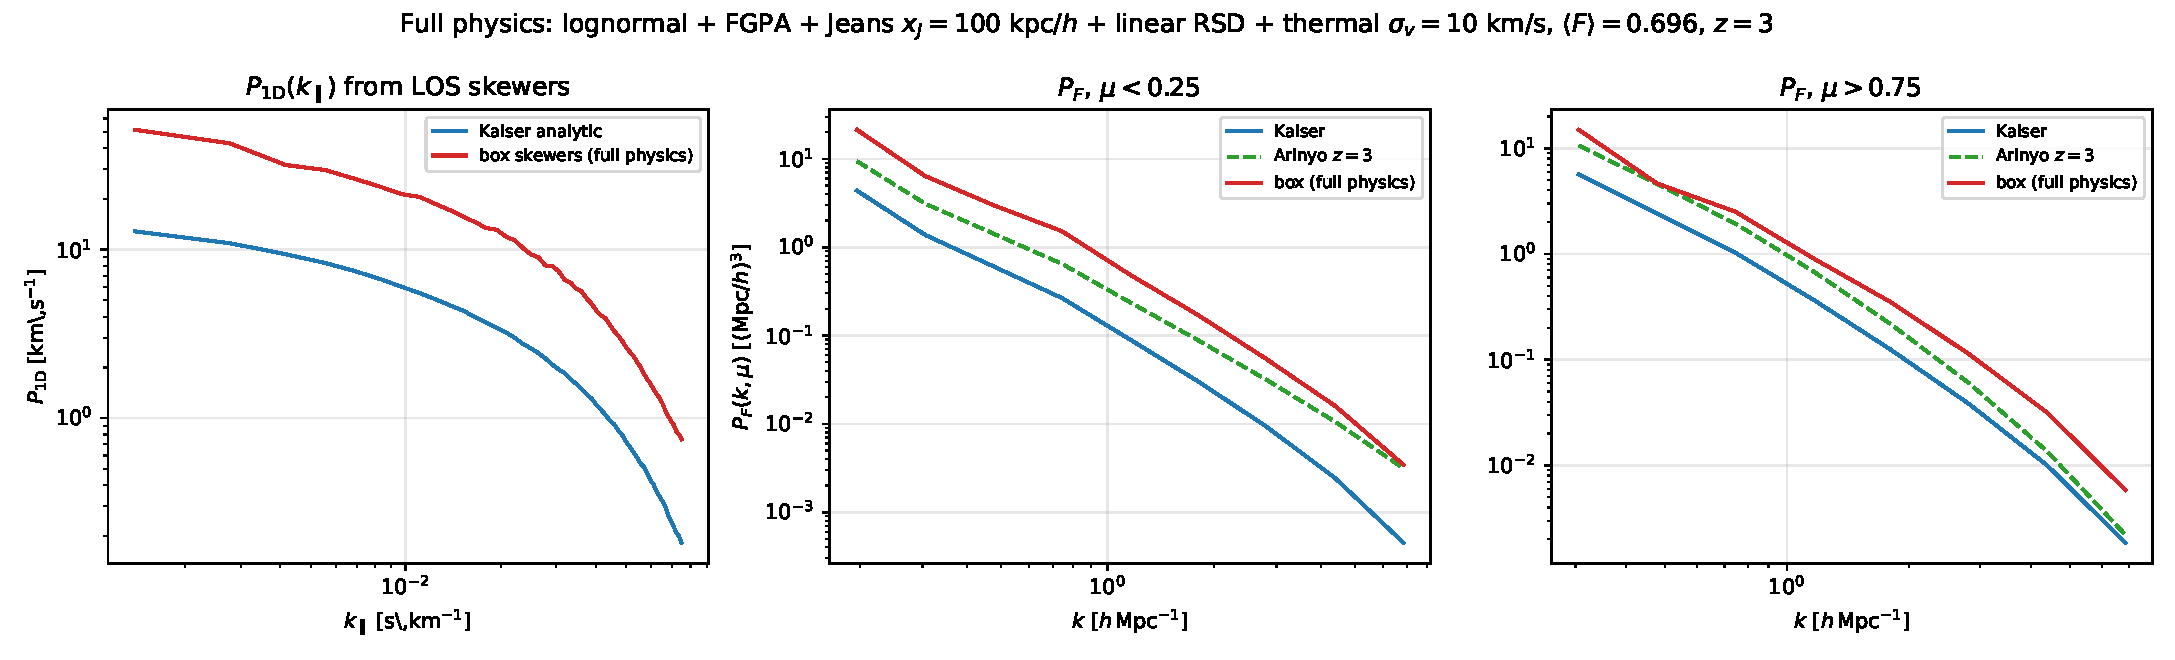
\includegraphics[width=\textwidth]{15_full_physics_p1d_p3d.pdf}
\caption{Full-physics measurement from one cube: lognormal FGPA, Jeans $x_J=100\,\mathrm{kpc}/h$, linear RSD, and thermal $\sigma_v=10\,\mathrm{km\,s}^{-1}$, at $\langle F\rangle=0.696$ and $z=3$.
Left: $P_{1\mathrm{D}}$ from all LOS skewers versus the analytic Kaiser projection.
Middle / right: $P_F(k,\mu)$ for mostly transverse and mostly parallel modes, with Kaiser and Arinyo-i-Prats overlays.}
\label{fig:fullphysics}
\end{figure}

As in Section~\ref{sec:box}, the lognormal amplitude lies above the fixed-bias Kaiser curve and above the published Arinyo formula; the slope remains closer to Arinyo than the amplitude does.
The main limits are unchanged: one small box, linear velocities only, and no refit of the Arinyo parameters.
Thermal broadening is now on, but the fiducial $10\,\mathrm{km\,s}^{-1}$ is only a fraction of a cell, so its effect is mild until $\sigma_v$ is raised (Figure~\ref{fig:paramvary}).

\subsection{Varying parameters}

Figure~\ref{fig:paramvary} repeats the full-physics cube while changing one parameter at a time, always measuring $P_{1\mathrm{D}}$ from the LOS skewers.
The four panels are $A_s$, $n_s$, the Jeans filter $\lambda_\mathrm{filter}\equiv x_J$, and the thermal width $\sigma_{v,\mathrm{th}}$.
The same random seed is kept so that changes in shape are not dominated by a new phase draw.

\begin{figure}[htbp]
\centering
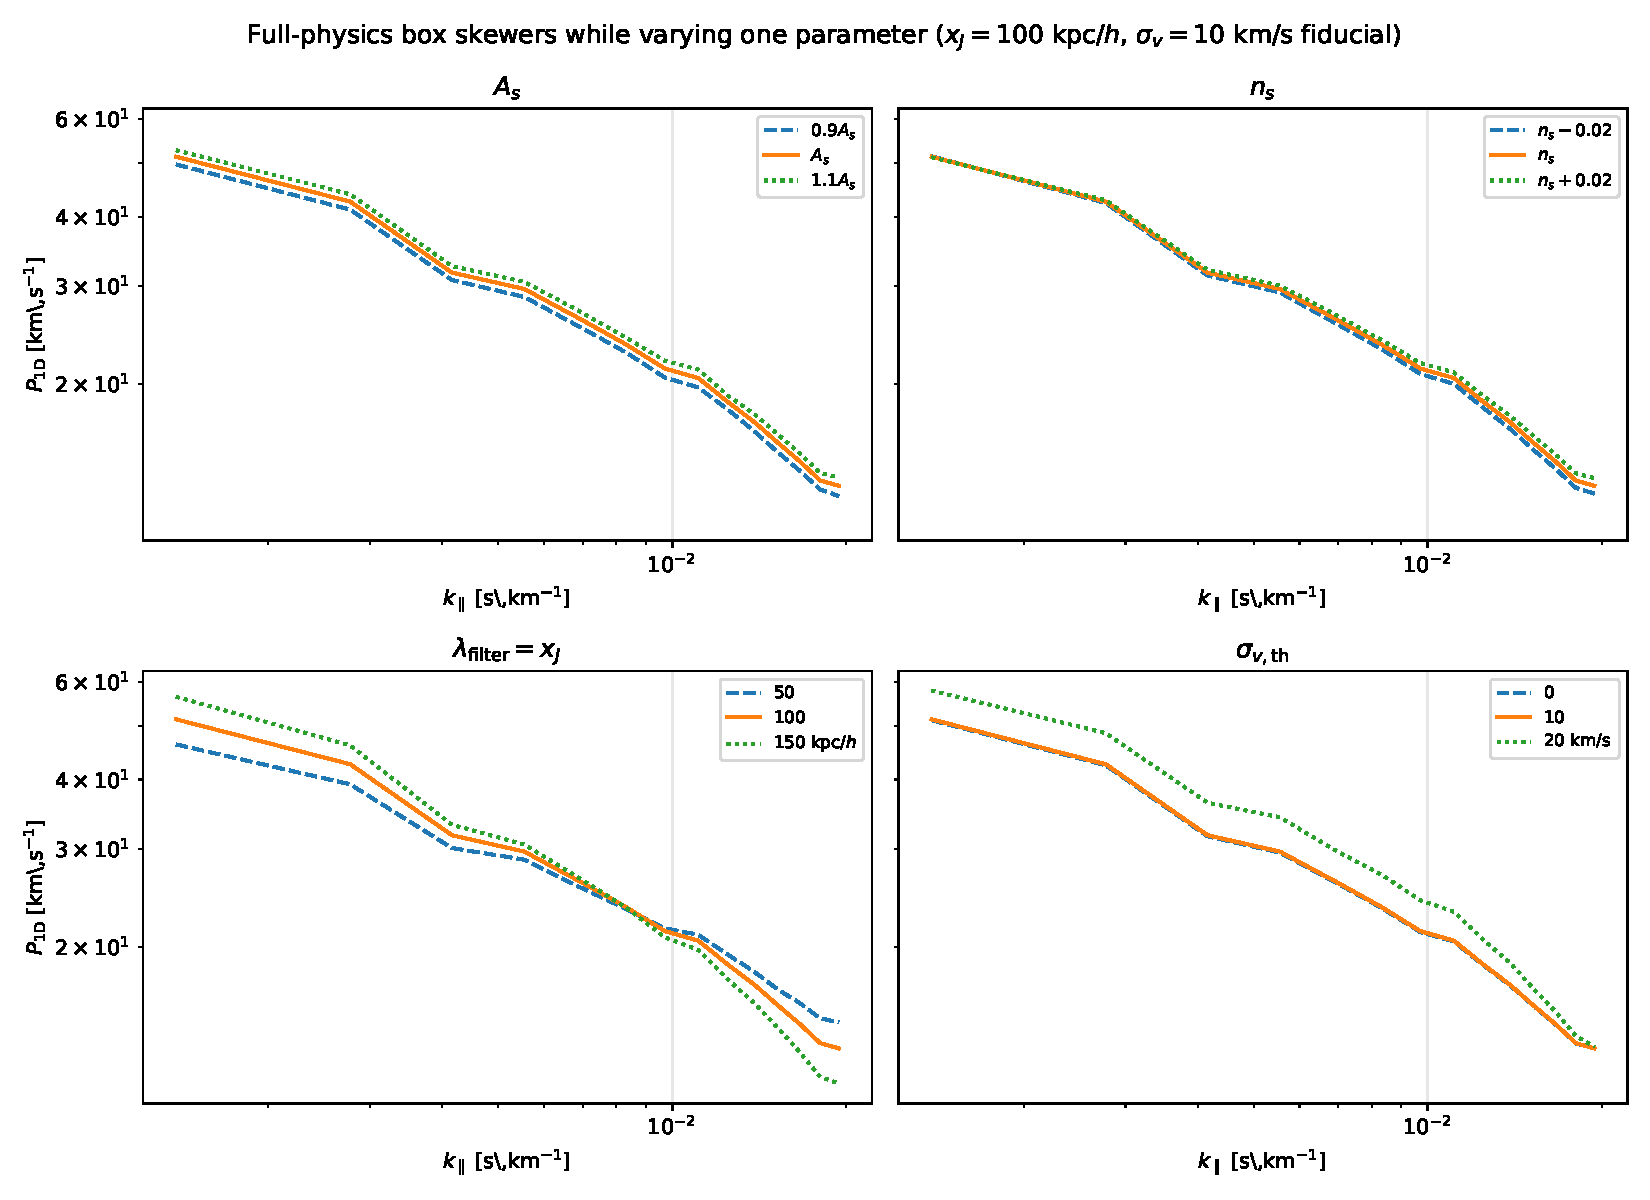
\includegraphics[width=\textwidth]{16_full_physics_param_vary.pdf}
\caption{Response of the full-physics box $P_{1\mathrm{D}}$ to one-parameter variations around the fiducial model of Figure~\ref{fig:fullphysics}.}
\label{fig:paramvary}
\end{figure}

\subsection{Code entry points}

\begin{center}
\small
\begin{tabular}{@{}p{0.42\textwidth}p{0.52\textwidth}@{}}
\toprule
Operation & Where \\
\midrule
Thermal width after RSD in the cube &
\texttt{fgpa\_flux\_box(..., thermal\_sigma\_mpch=...)} in \path{p1d/box3d.py} \\
Full-physics $P_{1\mathrm{D}}$ + $P_F(k,\mu)$ + variations &
\path{make\_full\_physics\_plots.py} \\
CLI knobs &
\texttt{--As}, \texttt{--ns}, \texttt{--lambda-filter}, \texttt{--thermal-kms}, \texttt{--mean-flux} \\
JAX twin of the pipeline (for later Fisher derivatives) &
\path{p1d\_jax/} (NumPy \path{p1d/} unchanged) \\
\bottomrule
\end{tabular}
\end{center}

Regenerate the figures with
\begin{verbatim}
python make_full_physics_plots.py
python make_full_physics_plots.py --As 2.3e-9 --ns 0.96 \
    --lambda-filter 0.1 --thermal-kms 10
\end{verbatim}


% Post-meeting full-physics upgrade (figures 15--16). Comment out if compiling without those PDFs.
% Overleaf drop-in note: upgrades after the Tuesday meeting (Kier / Vera / Simeon).
% Paste after the ``Three-dimensional flux power'' section of part2.tex, or
% % Overleaf drop-in note: upgrades after the Tuesday meeting (Kier / Vera / Simeon).
% Paste after the ``Three-dimensional flux power'' section of part2.tex, or
% % Overleaf drop-in note: upgrades after the Tuesday meeting (Kier / Vera / Simeon).
% Paste after the ``Three-dimensional flux power'' section of part2.tex, or
% \input{update_post_meeting} from the main file. Figures live in plots/.
%
% Companion script: make_full_physics_plots.py
% Figures: 15_full_physics_p1d_p3d.pdf, 16_full_physics_param_vary.pdf

\section{Post-meeting upgrade: full physics in one realisation}
\label{sec:fullphysics}

\subsection{Motivation}

The Tuesday discussion asked for $P_{1\mathrm{D}}(k_\parallel)$ and $P_F(k,\mu)$ measured from sightlines that include the same physics: lognormal density, Jeans smoothing, thermal broadening, FGPA optical depth, and peculiar velocities.
Section~\ref{sec:box} already had Jeans, lognormal, FGPA, and linear redshift-space distortions in the cube, but thermal broadening was off, and $P_{1\mathrm{D}}$ was not taken from that same volume.
The 1D FGPA sightlines of Part~I remained in real space.

\subsection{What changed relative to Figure~\ref{fig:box}}

\begin{center}
\small
\begin{tabular}{@{}lll@{}}
\toprule
Ingredient & Figure~\ref{fig:box} (meeting) & This update \\
\midrule
Jeans $x_J$ on $P_\mathrm{CDM}$ & $100\,\mathrm{kpc}/h$ & same \\
Lognormal $\Delta$ + FGPA $\tau=A\Delta^{\beta}$ & yes & same \\
Linear peculiar velocities (CIC on $\tau$) & yes & same \\
Thermal Gaussian on $\tau$ (after the shift) & off & on ($\sigma_v=10\,\mathrm{km\,s}^{-1}$ fiducial) \\
$\langle F\rangle$ & $0.696$ & same \\
$P_F(k,\mu)$ from the cube & yes & yes \\
$P_{1\mathrm{D}}$ from the same LOS skewers & no & yes \\
Parameter variations & no & $A_s$, $n_s$, $x_J$, $\sigma_{v,\mathrm{th}}$ \\
\bottomrule
\end{tabular}
\end{center}

The processing order in the cube is now
\begin{equation}
\delta_G
\;\to\;
\Delta=\mathrm{e}^{\delta_G-\sigma_G^{2}/2}
\;\to\;
\tau_\mathrm{unit}=\Delta^{\beta}
\;\to\;
\text{CIC shift by }\psi_\parallel
\;\to\;
\text{thermal smooth along the LOS}
\;\to\;
\text{solve }A\text{ so }\langle\mathrm{e}^{-A\tau}\rangle=\langle F\rangle.
\end{equation}
The thermal width is specified in $\mathrm{km\,s}^{-1}$ and converted to comoving $\mathrm{Mpc}/h$ with $H(z)/((1+z)h)$, then to pixels with the cell size $L/N$.
At $z=3$, $\sigma_v=10\,\mathrm{km\,s}^{-1}$ corresponds to $\sigma_x\approx 0.088\,\mathrm{Mpc}/h$ ($\sim 0.3$ cells on the $40\,\mathrm{Mpc}/h$, $128^{3}$ grid).

Every transverse cell provides one line-of-sight skewer.
$P_{1\mathrm{D}}$ is the ensemble periodogram of those $N^{2}$ flux-contrast skewers; $P_F(k,\mu)$ is the same 3D contrast binned in $k$ and $\mu$.
Both therefore share one seed, one Jeans length, one thermal width, and one fitted $A$.

\subsection{Fiducial measurement}

Figure~\ref{fig:fullphysics} uses the same geometry as Figure~\ref{fig:box}: $L=40\,\mathrm{Mpc}/h$, $N=128$, $z=3$, $x_J=100\,\mathrm{kpc}/h$, $\langle F\rangle=0.696$, linear growth rate $f\approx 0.982$.
The left panel is $P_{1\mathrm{D}}(k_\parallel)$ from the box skewers, with the analytic Kaiser $P_{1\mathrm{D}}$ on the Jeans-smoothed spectrum for reference.
The middle and right panels are $P_F(k,\mu)$ for $\mu<0.25$ and $\mu>0.75$, with the Part~I Kaiser formula and the published Arinyo-i-Prats $z=3$ formula overlaid (still not refitted).

\begin{figure}[htbp]
\centering
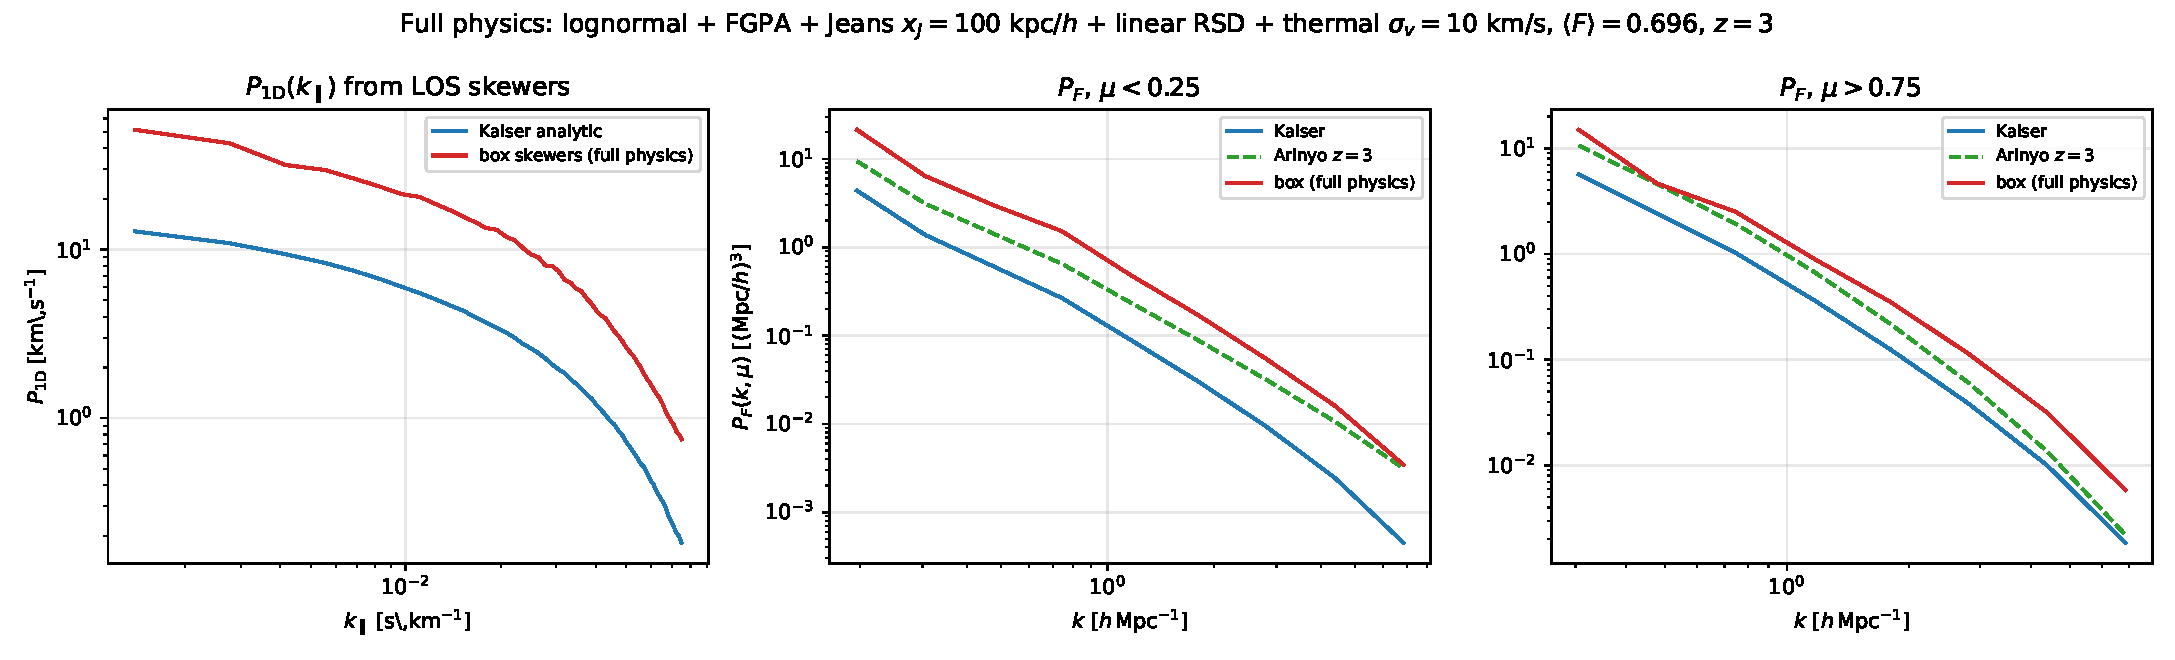
\includegraphics[width=\textwidth]{15_full_physics_p1d_p3d.pdf}
\caption{Full-physics measurement from one cube: lognormal FGPA, Jeans $x_J=100\,\mathrm{kpc}/h$, linear RSD, and thermal $\sigma_v=10\,\mathrm{km\,s}^{-1}$, at $\langle F\rangle=0.696$ and $z=3$.
Left: $P_{1\mathrm{D}}$ from all LOS skewers versus the analytic Kaiser projection.
Middle / right: $P_F(k,\mu)$ for mostly transverse and mostly parallel modes, with Kaiser and Arinyo-i-Prats overlays.}
\label{fig:fullphysics}
\end{figure}

As in Section~\ref{sec:box}, the lognormal amplitude lies above the fixed-bias Kaiser curve and above the published Arinyo formula; the slope remains closer to Arinyo than the amplitude does.
The main limits are unchanged: one small box, linear velocities only, and no refit of the Arinyo parameters.
Thermal broadening is now on, but the fiducial $10\,\mathrm{km\,s}^{-1}$ is only a fraction of a cell, so its effect is mild until $\sigma_v$ is raised (Figure~\ref{fig:paramvary}).

\subsection{Varying parameters}

Figure~\ref{fig:paramvary} repeats the full-physics cube while changing one parameter at a time, always measuring $P_{1\mathrm{D}}$ from the LOS skewers.
The four panels are $A_s$, $n_s$, the Jeans filter $\lambda_\mathrm{filter}\equiv x_J$, and the thermal width $\sigma_{v,\mathrm{th}}$.
The same random seed is kept so that changes in shape are not dominated by a new phase draw.

\begin{figure}[htbp]
\centering
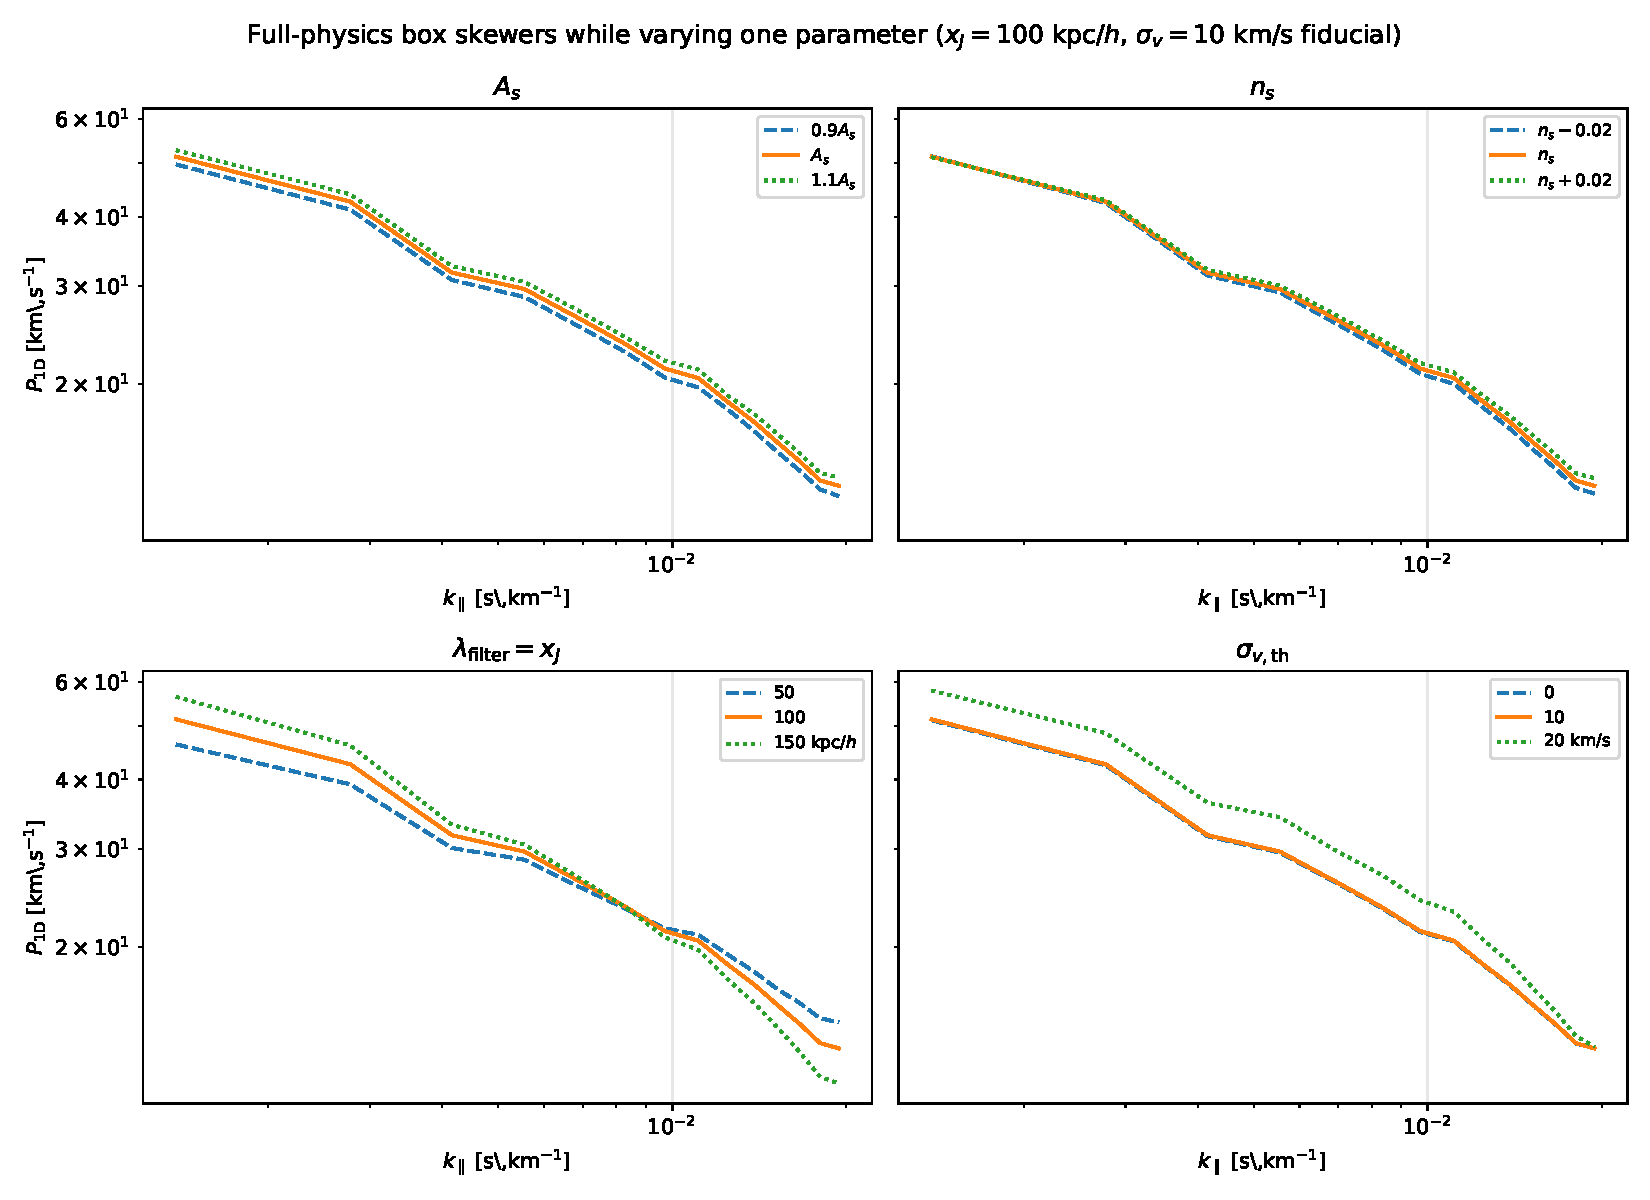
\includegraphics[width=\textwidth]{16_full_physics_param_vary.pdf}
\caption{Response of the full-physics box $P_{1\mathrm{D}}$ to one-parameter variations around the fiducial model of Figure~\ref{fig:fullphysics}.}
\label{fig:paramvary}
\end{figure}

\subsection{Code entry points}

\begin{center}
\small
\begin{tabular}{@{}p{0.42\textwidth}p{0.52\textwidth}@{}}
\toprule
Operation & Where \\
\midrule
Thermal width after RSD in the cube &
\texttt{fgpa\_flux\_box(..., thermal\_sigma\_mpch=...)} in \path{p1d/box3d.py} \\
Full-physics $P_{1\mathrm{D}}$ + $P_F(k,\mu)$ + variations &
\path{make\_full\_physics\_plots.py} \\
CLI knobs &
\texttt{--As}, \texttt{--ns}, \texttt{--lambda-filter}, \texttt{--thermal-kms}, \texttt{--mean-flux} \\
JAX twin of the pipeline (for later Fisher derivatives) &
\path{p1d\_jax/} (NumPy \path{p1d/} unchanged) \\
\bottomrule
\end{tabular}
\end{center}

Regenerate the figures with
\begin{verbatim}
python make_full_physics_plots.py
python make_full_physics_plots.py --As 2.3e-9 --ns 0.96 \
    --lambda-filter 0.1 --thermal-kms 10
\end{verbatim}
 from the main file. Figures live in plots/.
%
% Companion script: make_full_physics_plots.py
% Figures: 15_full_physics_p1d_p3d.pdf, 16_full_physics_param_vary.pdf

\section{Post-meeting upgrade: full physics in one realisation}
\label{sec:fullphysics}

\subsection{Motivation}

The Tuesday discussion asked for $P_{1\mathrm{D}}(k_\parallel)$ and $P_F(k,\mu)$ measured from sightlines that include the same physics: lognormal density, Jeans smoothing, thermal broadening, FGPA optical depth, and peculiar velocities.
Section~\ref{sec:box} already had Jeans, lognormal, FGPA, and linear redshift-space distortions in the cube, but thermal broadening was off, and $P_{1\mathrm{D}}$ was not taken from that same volume.
The 1D FGPA sightlines of Part~I remained in real space.

\subsection{What changed relative to Figure~\ref{fig:box}}

\begin{center}
\small
\begin{tabular}{@{}lll@{}}
\toprule
Ingredient & Figure~\ref{fig:box} (meeting) & This update \\
\midrule
Jeans $x_J$ on $P_\mathrm{CDM}$ & $100\,\mathrm{kpc}/h$ & same \\
Lognormal $\Delta$ + FGPA $\tau=A\Delta^{\beta}$ & yes & same \\
Linear peculiar velocities (CIC on $\tau$) & yes & same \\
Thermal Gaussian on $\tau$ (after the shift) & off & on ($\sigma_v=10\,\mathrm{km\,s}^{-1}$ fiducial) \\
$\langle F\rangle$ & $0.696$ & same \\
$P_F(k,\mu)$ from the cube & yes & yes \\
$P_{1\mathrm{D}}$ from the same LOS skewers & no & yes \\
Parameter variations & no & $A_s$, $n_s$, $x_J$, $\sigma_{v,\mathrm{th}}$ \\
\bottomrule
\end{tabular}
\end{center}

The processing order in the cube is now
\begin{equation}
\delta_G
\;\to\;
\Delta=\mathrm{e}^{\delta_G-\sigma_G^{2}/2}
\;\to\;
\tau_\mathrm{unit}=\Delta^{\beta}
\;\to\;
\text{CIC shift by }\psi_\parallel
\;\to\;
\text{thermal smooth along the LOS}
\;\to\;
\text{solve }A\text{ so }\langle\mathrm{e}^{-A\tau}\rangle=\langle F\rangle.
\end{equation}
The thermal width is specified in $\mathrm{km\,s}^{-1}$ and converted to comoving $\mathrm{Mpc}/h$ with $H(z)/((1+z)h)$, then to pixels with the cell size $L/N$.
At $z=3$, $\sigma_v=10\,\mathrm{km\,s}^{-1}$ corresponds to $\sigma_x\approx 0.088\,\mathrm{Mpc}/h$ ($\sim 0.3$ cells on the $40\,\mathrm{Mpc}/h$, $128^{3}$ grid).

Every transverse cell provides one line-of-sight skewer.
$P_{1\mathrm{D}}$ is the ensemble periodogram of those $N^{2}$ flux-contrast skewers; $P_F(k,\mu)$ is the same 3D contrast binned in $k$ and $\mu$.
Both therefore share one seed, one Jeans length, one thermal width, and one fitted $A$.

\subsection{Fiducial measurement}

Figure~\ref{fig:fullphysics} uses the same geometry as Figure~\ref{fig:box}: $L=40\,\mathrm{Mpc}/h$, $N=128$, $z=3$, $x_J=100\,\mathrm{kpc}/h$, $\langle F\rangle=0.696$, linear growth rate $f\approx 0.982$.
The left panel is $P_{1\mathrm{D}}(k_\parallel)$ from the box skewers, with the analytic Kaiser $P_{1\mathrm{D}}$ on the Jeans-smoothed spectrum for reference.
The middle and right panels are $P_F(k,\mu)$ for $\mu<0.25$ and $\mu>0.75$, with the Part~I Kaiser formula and the published Arinyo-i-Prats $z=3$ formula overlaid (still not refitted).

\begin{figure}[htbp]
\centering
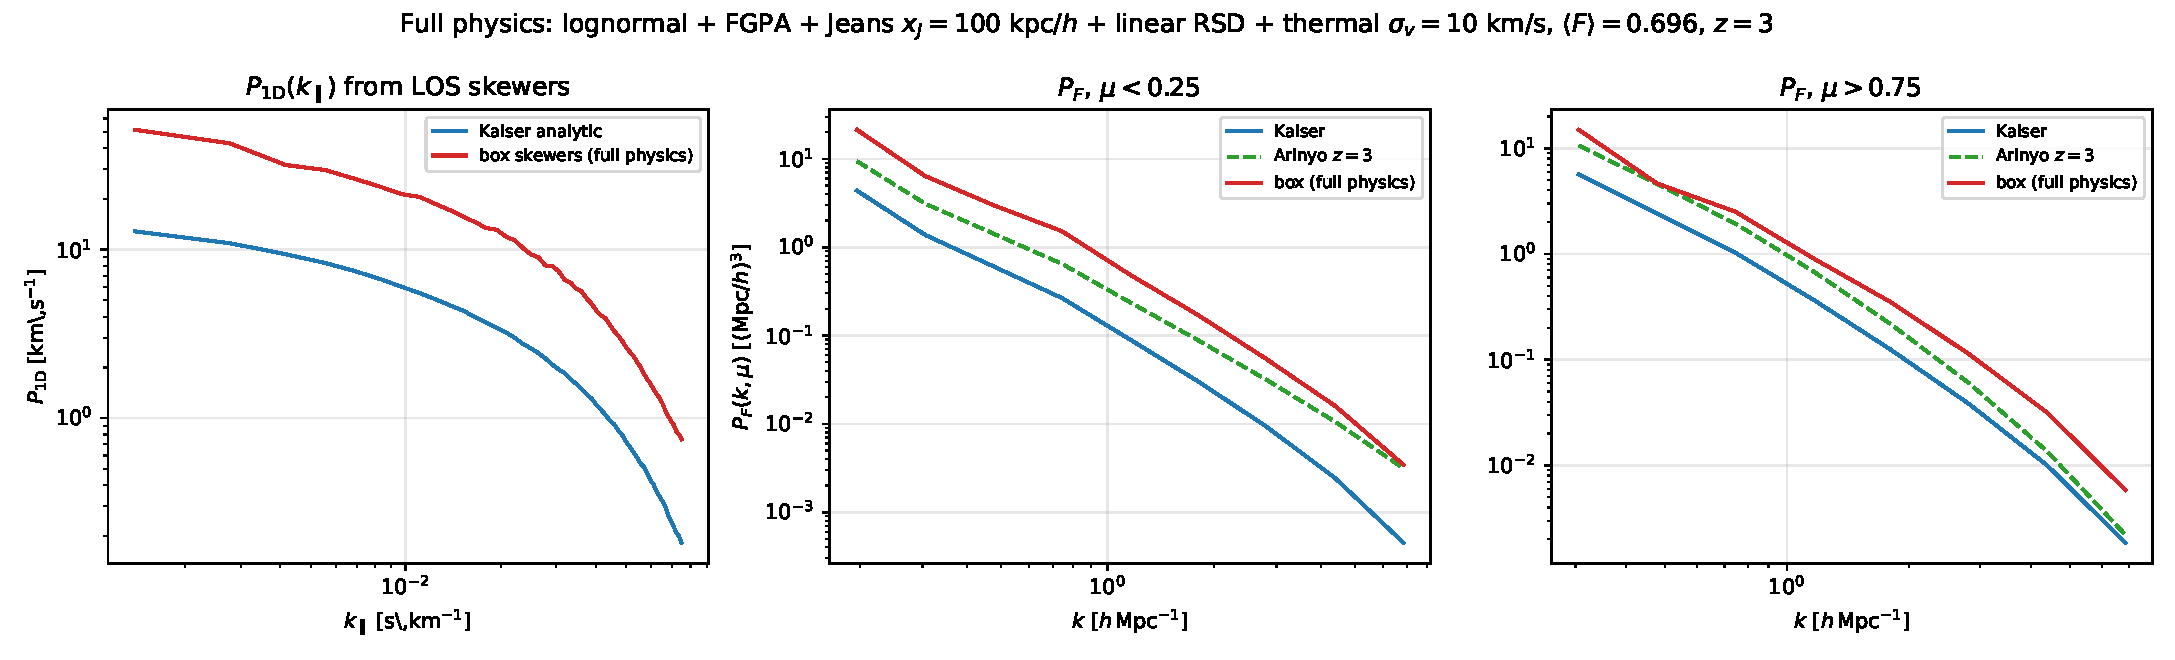
\includegraphics[width=\textwidth]{15_full_physics_p1d_p3d.pdf}
\caption{Full-physics measurement from one cube: lognormal FGPA, Jeans $x_J=100\,\mathrm{kpc}/h$, linear RSD, and thermal $\sigma_v=10\,\mathrm{km\,s}^{-1}$, at $\langle F\rangle=0.696$ and $z=3$.
Left: $P_{1\mathrm{D}}$ from all LOS skewers versus the analytic Kaiser projection.
Middle / right: $P_F(k,\mu)$ for mostly transverse and mostly parallel modes, with Kaiser and Arinyo-i-Prats overlays.}
\label{fig:fullphysics}
\end{figure}

As in Section~\ref{sec:box}, the lognormal amplitude lies above the fixed-bias Kaiser curve and above the published Arinyo formula; the slope remains closer to Arinyo than the amplitude does.
The main limits are unchanged: one small box, linear velocities only, and no refit of the Arinyo parameters.
Thermal broadening is now on, but the fiducial $10\,\mathrm{km\,s}^{-1}$ is only a fraction of a cell, so its effect is mild until $\sigma_v$ is raised (Figure~\ref{fig:paramvary}).

\subsection{Varying parameters}

Figure~\ref{fig:paramvary} repeats the full-physics cube while changing one parameter at a time, always measuring $P_{1\mathrm{D}}$ from the LOS skewers.
The four panels are $A_s$, $n_s$, the Jeans filter $\lambda_\mathrm{filter}\equiv x_J$, and the thermal width $\sigma_{v,\mathrm{th}}$.
The same random seed is kept so that changes in shape are not dominated by a new phase draw.

\begin{figure}[htbp]
\centering
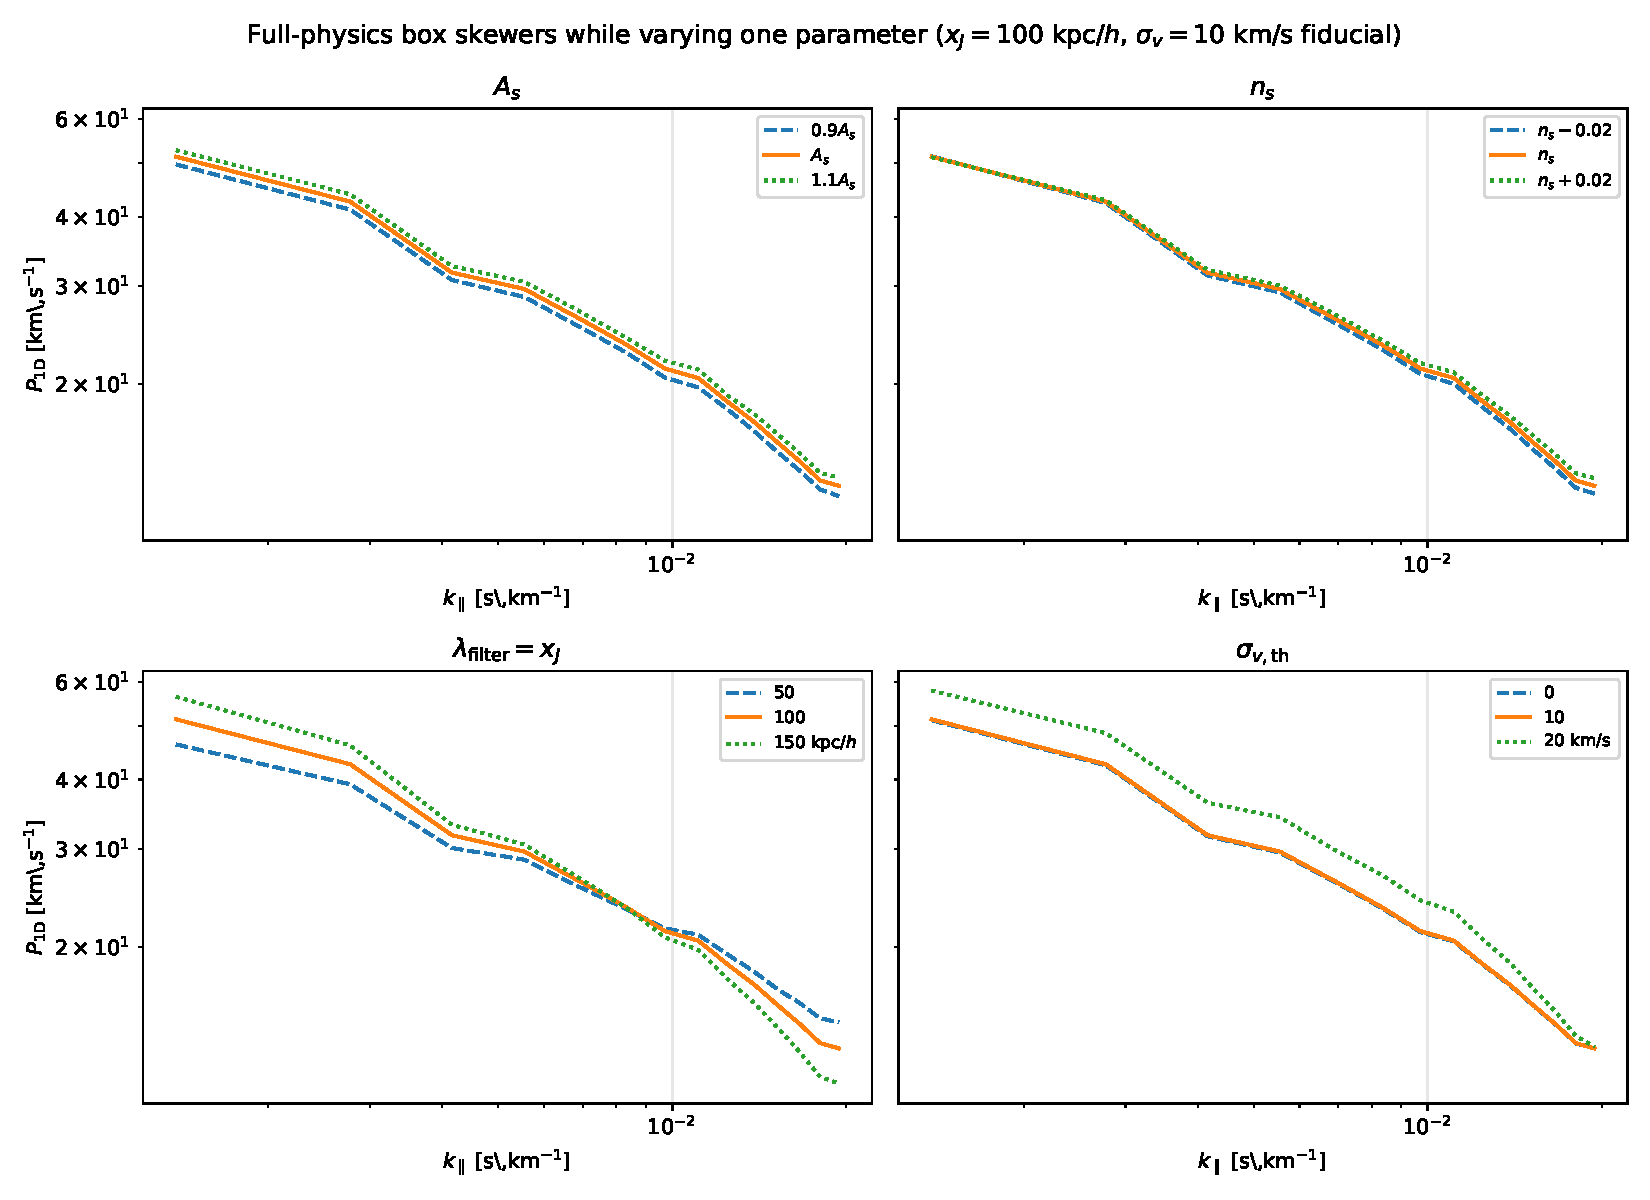
\includegraphics[width=\textwidth]{16_full_physics_param_vary.pdf}
\caption{Response of the full-physics box $P_{1\mathrm{D}}$ to one-parameter variations around the fiducial model of Figure~\ref{fig:fullphysics}.}
\label{fig:paramvary}
\end{figure}

\subsection{Code entry points}

\begin{center}
\small
\begin{tabular}{@{}p{0.42\textwidth}p{0.52\textwidth}@{}}
\toprule
Operation & Where \\
\midrule
Thermal width after RSD in the cube &
\texttt{fgpa\_flux\_box(..., thermal\_sigma\_mpch=...)} in \path{p1d/box3d.py} \\
Full-physics $P_{1\mathrm{D}}$ + $P_F(k,\mu)$ + variations &
\path{make\_full\_physics\_plots.py} \\
CLI knobs &
\texttt{--As}, \texttt{--ns}, \texttt{--lambda-filter}, \texttt{--thermal-kms}, \texttt{--mean-flux} \\
JAX twin of the pipeline (for later Fisher derivatives) &
\path{p1d\_jax/} (NumPy \path{p1d/} unchanged) \\
\bottomrule
\end{tabular}
\end{center}

Regenerate the figures with
\begin{verbatim}
python make_full_physics_plots.py
python make_full_physics_plots.py --As 2.3e-9 --ns 0.96 \
    --lambda-filter 0.1 --thermal-kms 10
\end{verbatim}
 from the main file. Figures live in plots/.
%
% Companion script: make_full_physics_plots.py
% Figures: 15_full_physics_p1d_p3d.pdf, 16_full_physics_param_vary.pdf

\section{Post-meeting upgrade: full physics in one realisation}
\label{sec:fullphysics}

\subsection{Motivation}

The Tuesday discussion asked for $P_{1\mathrm{D}}(k_\parallel)$ and $P_F(k,\mu)$ measured from sightlines that include the same physics: lognormal density, Jeans smoothing, thermal broadening, FGPA optical depth, and peculiar velocities.
Section~\ref{sec:box} already had Jeans, lognormal, FGPA, and linear redshift-space distortions in the cube, but thermal broadening was off, and $P_{1\mathrm{D}}$ was not taken from that same volume.
The 1D FGPA sightlines of Part~I remained in real space.

\subsection{What changed relative to Figure~\ref{fig:box}}

\begin{center}
\small
\begin{tabular}{@{}lll@{}}
\toprule
Ingredient & Figure~\ref{fig:box} (meeting) & This update \\
\midrule
Jeans $x_J$ on $P_\mathrm{CDM}$ & $100\,\mathrm{kpc}/h$ & same \\
Lognormal $\Delta$ + FGPA $\tau=A\Delta^{\beta}$ & yes & same \\
Linear peculiar velocities (CIC on $\tau$) & yes & same \\
Thermal Gaussian on $\tau$ (after the shift) & off & on ($\sigma_v=10\,\mathrm{km\,s}^{-1}$ fiducial) \\
$\langle F\rangle$ & $0.696$ & same \\
$P_F(k,\mu)$ from the cube & yes & yes \\
$P_{1\mathrm{D}}$ from the same LOS skewers & no & yes \\
Parameter variations & no & $A_s$, $n_s$, $x_J$, $\sigma_{v,\mathrm{th}}$ \\
\bottomrule
\end{tabular}
\end{center}

The processing order in the cube is now
\begin{equation}
\delta_G
\;\to\;
\Delta=\mathrm{e}^{\delta_G-\sigma_G^{2}/2}
\;\to\;
\tau_\mathrm{unit}=\Delta^{\beta}
\;\to\;
\text{CIC shift by }\psi_\parallel
\;\to\;
\text{thermal smooth along the LOS}
\;\to\;
\text{solve }A\text{ so }\langle\mathrm{e}^{-A\tau}\rangle=\langle F\rangle.
\end{equation}
The thermal width is specified in $\mathrm{km\,s}^{-1}$ and converted to comoving $\mathrm{Mpc}/h$ with $H(z)/((1+z)h)$, then to pixels with the cell size $L/N$.
At $z=3$, $\sigma_v=10\,\mathrm{km\,s}^{-1}$ corresponds to $\sigma_x\approx 0.088\,\mathrm{Mpc}/h$ ($\sim 0.3$ cells on the $40\,\mathrm{Mpc}/h$, $128^{3}$ grid).

Every transverse cell provides one line-of-sight skewer.
$P_{1\mathrm{D}}$ is the ensemble periodogram of those $N^{2}$ flux-contrast skewers; $P_F(k,\mu)$ is the same 3D contrast binned in $k$ and $\mu$.
Both therefore share one seed, one Jeans length, one thermal width, and one fitted $A$.

\subsection{Fiducial measurement}

Figure~\ref{fig:fullphysics} uses the same geometry as Figure~\ref{fig:box}: $L=40\,\mathrm{Mpc}/h$, $N=128$, $z=3$, $x_J=100\,\mathrm{kpc}/h$, $\langle F\rangle=0.696$, linear growth rate $f\approx 0.982$.
The left panel is $P_{1\mathrm{D}}(k_\parallel)$ from the box skewers, with the analytic Kaiser $P_{1\mathrm{D}}$ on the Jeans-smoothed spectrum for reference.
The middle and right panels are $P_F(k,\mu)$ for $\mu<0.25$ and $\mu>0.75$, with the Part~I Kaiser formula and the published Arinyo-i-Prats $z=3$ formula overlaid (still not refitted).

\begin{figure}[htbp]
\centering
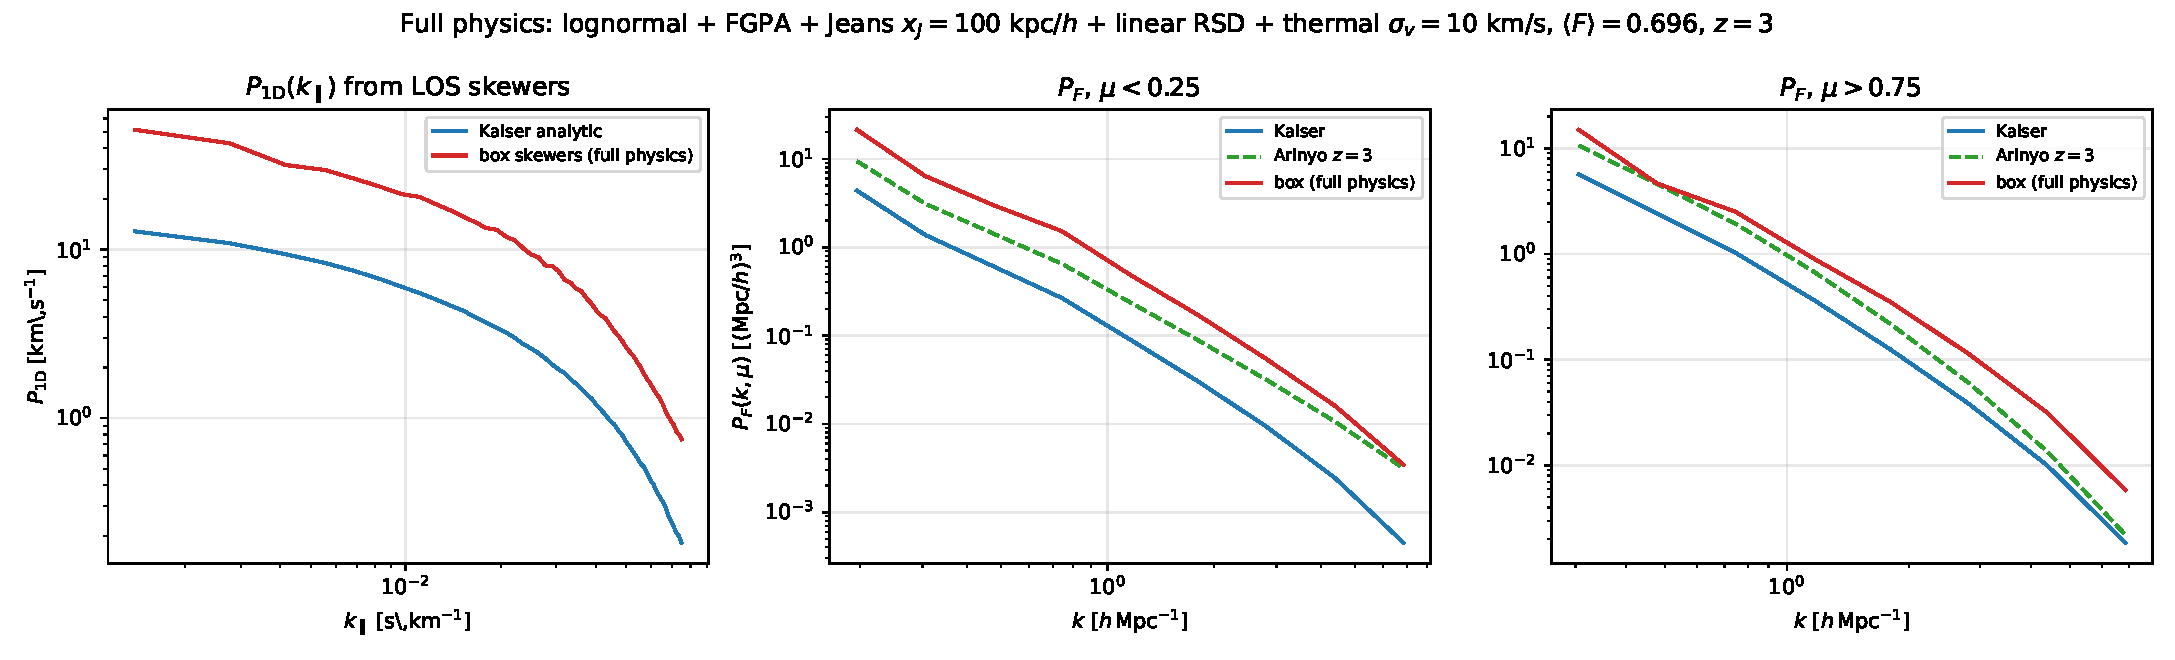
\includegraphics[width=\textwidth]{15_full_physics_p1d_p3d.pdf}
\caption{Full-physics measurement from one cube: lognormal FGPA, Jeans $x_J=100\,\mathrm{kpc}/h$, linear RSD, and thermal $\sigma_v=10\,\mathrm{km\,s}^{-1}$, at $\langle F\rangle=0.696$ and $z=3$.
Left: $P_{1\mathrm{D}}$ from all LOS skewers versus the analytic Kaiser projection.
Middle / right: $P_F(k,\mu)$ for mostly transverse and mostly parallel modes, with Kaiser and Arinyo-i-Prats overlays.}
\label{fig:fullphysics}
\end{figure}

As in Section~\ref{sec:box}, the lognormal amplitude lies above the fixed-bias Kaiser curve and above the published Arinyo formula; the slope remains closer to Arinyo than the amplitude does.
The main limits are unchanged: one small box, linear velocities only, and no refit of the Arinyo parameters.
Thermal broadening is now on, but the fiducial $10\,\mathrm{km\,s}^{-1}$ is only a fraction of a cell, so its effect is mild until $\sigma_v$ is raised (Figure~\ref{fig:paramvary}).

\subsection{Varying parameters}

Figure~\ref{fig:paramvary} repeats the full-physics cube while changing one parameter at a time, always measuring $P_{1\mathrm{D}}$ from the LOS skewers.
The four panels are $A_s$, $n_s$, the Jeans filter $\lambda_\mathrm{filter}\equiv x_J$, and the thermal width $\sigma_{v,\mathrm{th}}$.
The same random seed is kept so that changes in shape are not dominated by a new phase draw.

\begin{figure}[htbp]
\centering
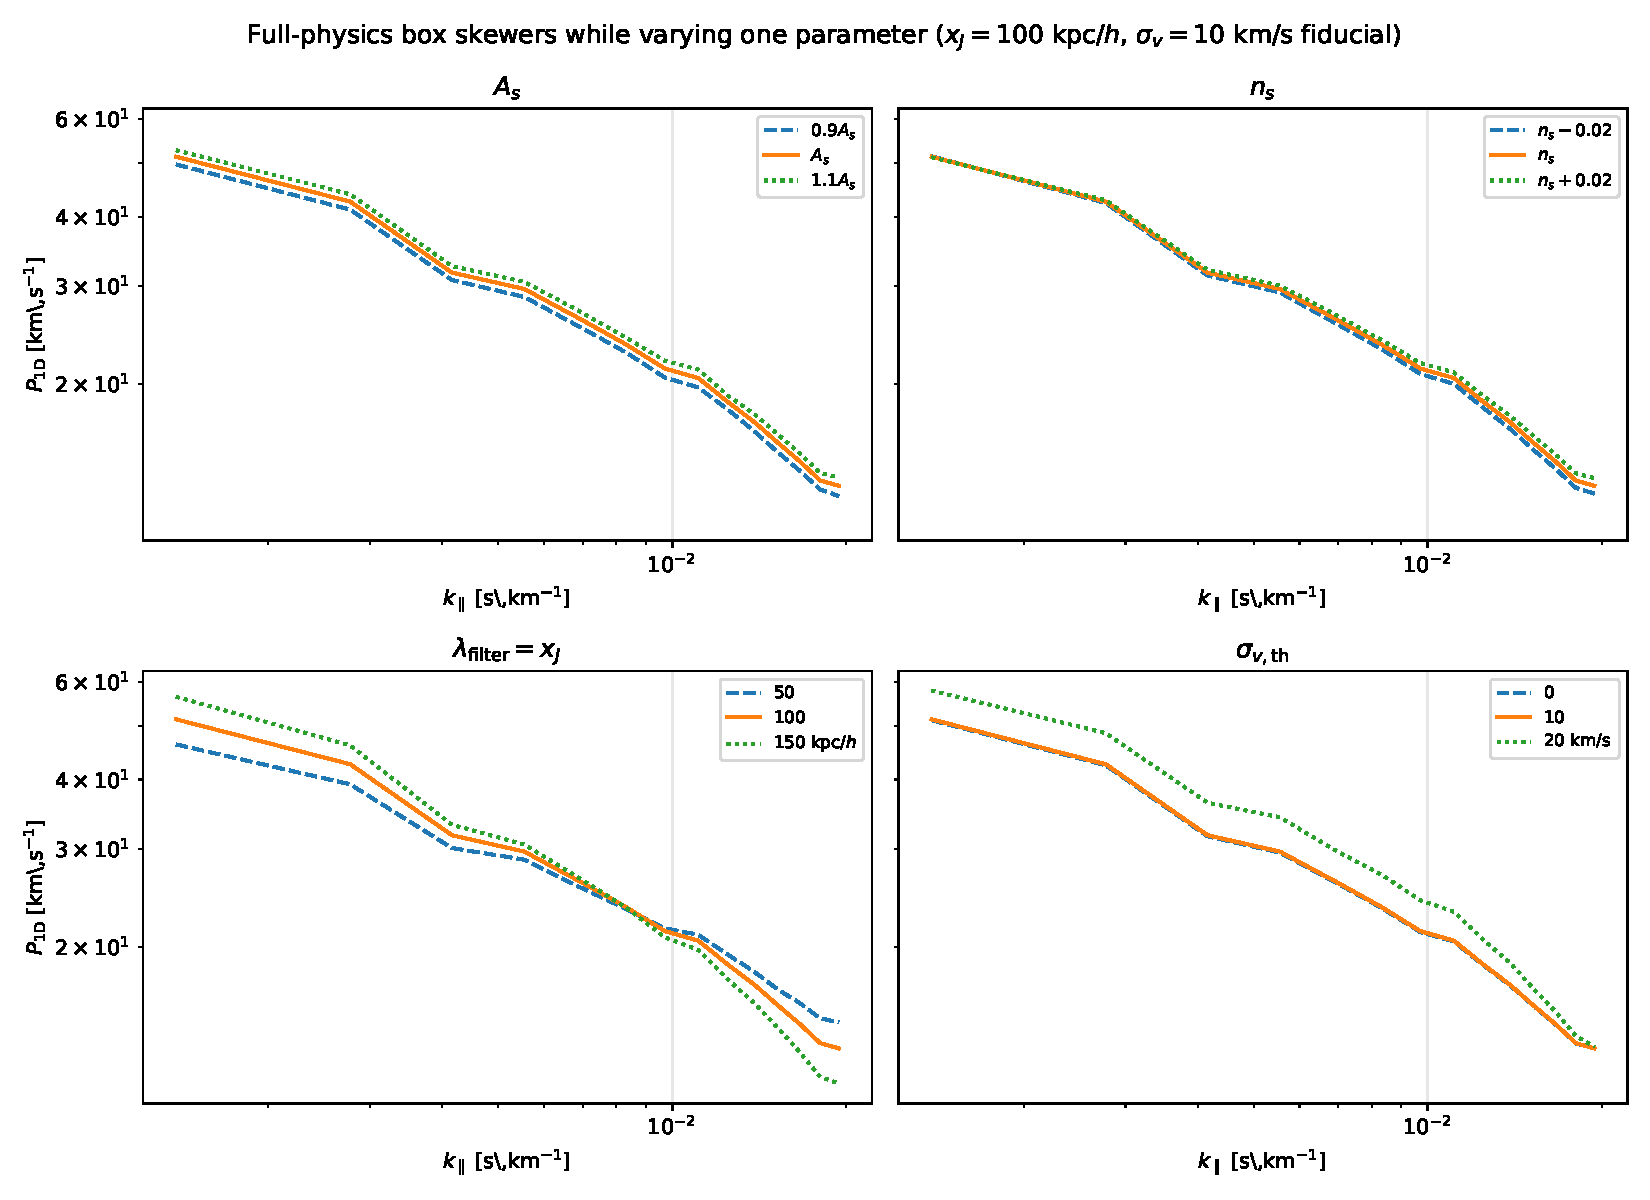
\includegraphics[width=\textwidth]{16_full_physics_param_vary.pdf}
\caption{Response of the full-physics box $P_{1\mathrm{D}}$ to one-parameter variations around the fiducial model of Figure~\ref{fig:fullphysics}.}
\label{fig:paramvary}
\end{figure}

\subsection{Code entry points}

\begin{center}
\small
\begin{tabular}{@{}p{0.42\textwidth}p{0.52\textwidth}@{}}
\toprule
Operation & Where \\
\midrule
Thermal width after RSD in the cube &
\texttt{fgpa\_flux\_box(..., thermal\_sigma\_mpch=...)} in \path{p1d/box3d.py} \\
Full-physics $P_{1\mathrm{D}}$ + $P_F(k,\mu)$ + variations &
\path{make\_full\_physics\_plots.py} \\
CLI knobs &
\texttt{--As}, \texttt{--ns}, \texttt{--lambda-filter}, \texttt{--thermal-kms}, \texttt{--mean-flux} \\
JAX twin of the pipeline (for later Fisher derivatives) &
\path{p1d\_jax/} (NumPy \path{p1d/} unchanged) \\
\bottomrule
\end{tabular}
\end{center}

Regenerate the figures with
\begin{verbatim}
python make_full_physics_plots.py
python make_full_physics_plots.py --As 2.3e-9 --ns 0.96 \
    --lambda-filter 0.1 --thermal-kms 10
\end{verbatim}


\section{Equations and sources}
\label{sec:sources}

\begin{center}
\small
\begin{tabular}{@{}p{0.42\textwidth}p{0.48\textwidth}@{}}
\toprule
Equation & Source \\
\midrule
Eisenstein--Hu $T(k)$ and $P_\mathrm{CDM}$ &
\cite{Eisenstein:1997ik}; Part~I \\
Kaiser factor \eqref{eq:kaiser} &
\cite{Kaiser:1987qv,McDonald:2001fe}; $b_F$, $\beta_F$ from \cite{Gordon:2023dua} \\
Line-of-sight integral \eqref{eq:p1d} &
\cite{McDonald:2001fe}; Part~I \\
Lognormal map \eqref{eq:lognormal} &
\cite{Coles:1991if,Bi:1996fh,Arya:2022uke} \\
Optical depth \eqref{eq:fgpa} &
\cite{Gunn:1965hd,Hui:1997dp} \\
Jeans factor \eqref{eq:jeans} &
\cite{Arya:2022uke} \\
Mean transmission \eqref{eq:taueff} &
\cite{Faucher-Giguere:2007ab}; extrapolated at $z=5$ \\
Nonlinear flux model \eqref{eq:arinyo}--\eqref{eq:btau} &
\cite{Arinyo-i-Prats:2015vqa}, Tables~2--3 at $z=3$, $q_2=0$ \\
Linear displacement \eqref{eq:disp} &
continuity equation; $f$ from Part~I growth \\
\bottomrule
\end{tabular}
\end{center}

\section{Implementation and how to run}
\label{sec:code}

The repository is \path{fisher-forecasts-future-spectroscopic-survey}.
Part~I lives in \path{p1d/}.
Nothing in Part~I is removed or rewritten.
The new modules are \path{p1d/jeans.py}, \path{p1d/arinyo.py}, and \path{p1d/box3d.py}.
Figures~09--12 are written by \path{make_extension_plots.py}.
Figures~13--14 are written by \path{make_meeting_plots.py}.
From the repository root,
\begin{verbatim}
python make_extension_plots.py
python make_meeting_plots.py
python -m pytest -q
\end{verbatim}
produce the figures and run the tests.
The Jeans, Arinyo, and box tests are in \path{tests/test_jeans.py}, \path{tests/test_arinyo.py}, and \path{tests/test_box3d.py}.

\subsection{The cutoff}

\texttt{jeans\_suppression(k, x\_j)} returns $\exp(-2 x_J^{2} k^{2})$ on the array $k$.
A zero length returns an array of ones; a negative length is rejected.
\texttt{with\_jeans(table, x\_j)} evaluates that factor on the wavenumber column of a \texttt{TabulatedMatterPower}, multiplies the stored power by it, and returns a new table.
The fiducial $A_s$, $n_s$, and pivot of the input table are copied onto the new one, so the Part~I rescaling still applies.
The input object is left unchanged.
A vanishing $x_J$ is the identity; $x_J=0.10\,\mathrm{Mpc}/h$ suppresses $k=10\,h\,\mathrm{Mpc}^{-1}$ relative to $k=10^{-3}\,h\,\mathrm{Mpc}^{-1}$.

The base table for figures~09--12 is built by \texttt{TabulatedMatterPower.from\_eisenstein\_hu} at the fiducial cosmology, with $k$ from $10^{-3}$ to $120\,h\,\mathrm{Mpc}^{-1}$ and $4000$ logarithmically spaced samples.
For $x_J=0$ the figure code passes this table through; for either positive length it passes the object returned by \texttt{with\_jeans}.

\subsection{Analytic flux on a screened spectrum}

\texttt{p1d\_skm} accepts an optional argument \texttt{matter\_power}.
When that argument is supplied, \texttt{flux\_power\_1d} evaluates it on the $800$ quadrature nodes in place of \texttt{linear\_matter\_power}.
The Kaiser factor and the trapezoidal integral are the Part~I functions.
In figure~11 the callable is the screened table, passed as \texttt{matter\_power}.
Redshift, $\Omega_m$, and $h$ still convert the result to $\mathrm{km\,s}^{-1}$.

Figure~09 does not use that integral.
Its unsmoothed curves call \texttt{flux\_power\_3d}, which multiplies the direct Eisenstein--Hu spectrum by $b_F^{2}(1+\beta_F\mu^{2})^{2}$.
Its smoothed curve multiplies the screened table, evaluated at $\mu=1$, by the same prefactor $(-0.14)^{2}(1+1.4)^{2}$.

\subsection{Sightlines on a screened spectrum}

The extension scripts draw lines with the Part~I primitives, in the following order (the same sequence that \texttt{run\_fgpa\_skewers} performs):

\begin{enumerate}
\item \texttt{rfft\_modes(L, N)} returns $k_j=2\pi j/L$, including the Nyquist mode.
\item The screened table is evaluated on $8192$ logarithmically spaced wavenumbers between its first and last entries, at the fiducial $A_s$ and $n_s$.
When the table is stored at the evaluation redshift, the growth ratio is unity.
\item \texttt{project\_p1d} integrates $q\,P_\mathrm{CDM}(q)$ from each line mode up to the last tabulated $k$.
\item \texttt{generate\_gaussian\_skewers} draws complex Gaussian coefficients with variance $N^{2}P_{1\mathrm{D}}/L$, sets the zero mode to zero, and returns the real field by an inverse transform.
\item \texttt{lognormal\_density} applies Eq.~\eqref{eq:lognormal}, using the variance of the lines just drawn.
\item For a flux spectrum, \texttt{prepare\_tau\_unit} raises the density to $\beta=\texttt{fgpa\_exponent}(1.5)=1.65$.
No displacement is passed, and the thermal width is left at zero.
The pixel smoother \texttt{smooth\_periodic} is not called, so the only suppression of small-scale power is Eq.~\eqref{eq:jeans}.
\item \texttt{calibrate\_mean\_flux} solves $\langle e^{-A\tau}\rangle=\langle F\rangle_\mathrm{target}$ for $\ln A$.
\texttt{transmitted\_flux} and \texttt{flux\_contrast} form $F$ and $\delta_F$.
\item \texttt{measure\_p1d} returns $(\mathrm{d}x)^{2}/L$ times the mean of $|\tilde\delta_F|^{2}$, and \texttt{p1d\_h\_to\_kms} converts that spectrum to $\mathrm{km\,s}^{-1}$.
\end{enumerate}

Figure~10 stops after the fifth step and measures the periodogram of $\delta_G$ and of $\Delta-1$.
Figure~11 continues through the eighth step.
Figure~12 uses the unsmoothed table, $L=200\,\mathrm{Mpc}/h$, $N=512$, and $10\,000$ lines; it stores the transmitted flux of the whole draw and repeats the contrast and the periodogram on slices of that array.
The Kaiser curve on that figure is \texttt{p1d\_skm} with its default matter spectrum.

\subsection{Redshift five and the cube}

Figure~13 calls the same line-drawing sequence at $z=5$, with $256$ lines, and passes the screened table into \texttt{flux\_power\_1d} with the quadrature limit set to $80\,h\,\mathrm{Mpc}^{-1}$.
The mean transmission is Eq.~\eqref{eq:taueff}.

Figure~14 is built in \path{p1d/box3d.py}.
\texttt{gaussian\_box} draws a periodic Gaussian field on $128^{3}$ cells.
The variance of each complex coefficient is $N^{6}P(k)/L^{3}$, which is the convention in which \texttt{measure\_power} returns $P(k)$.
Modes are paired so that the field is real, and the zero mode is zero.
For this figure the modulus of each coefficient is the rms and only the phase is random.
\texttt{kaiser\_flux\_from\_density} multiplies those coefficients by $b_F(1+\beta_F\mu^{2})$.
\texttt{fgpa\_flux\_box} applies Eq.~\eqref{eq:lognormal}, raises the density to $\beta=1.65$, shifts the optical depth with \texttt{los\_displacement} \eqref{eq:disp} and a cloud-in-cell deposit along the last axis, then solves for $A$.
\texttt{bin\_power} averages the mode-by-mode power in bins of $k$ and $\mu$.
The Arinyo-i-Prats curve is \texttt{flux\_power} in \path{p1d/arinyo.py}, which evaluates Eqs.~\eqref{eq:arinyo}--\eqref{eq:btau} at the published $z=3$ numbers.

\begin{center}
\small
\begin{tabular}{@{}p{0.42\textwidth}p{0.52\textwidth}@{}}
\toprule
Operation & Where it is implemented \\
\midrule
Equation~\eqref{eq:jeans} &
\texttt{jeans\_suppression} in \path{p1d/jeans.py} \\
New table, input left unchanged &
\texttt{with\_jeans} in \path{p1d/jeans.py} \\
Kaiser $P_F(k,\mu)$ on a grid &
\texttt{flux\_power\_3d} in \path{p1d/flux.py} \\
Kaiser $P_{1\mathrm{D}}$ of a screened table &
\texttt{p1d\_skm} with \texttt{matter\_power} set \\
Isotropic projection and Gaussian lines &
\texttt{project\_p1d}, \texttt{generate\_gaussian\_skewers} \\
Equations~\eqref{eq:lognormal}--\eqref{eq:fgpa} &
\texttt{lognormal\_density}, \texttt{prepare\_tau\_unit}, \texttt{calibrate\_mean\_flux} \\
Sightline $P_{1\mathrm{D}}$ &
\texttt{measure\_p1d}, then \texttt{p1d\_h\_to\_kms} \\
Figures 09--12 &
\path{make_extension_plots.py} \\
Equations~\eqref{eq:arinyo}--\eqref{eq:btau} &
\texttt{flux\_power} in \path{p1d/arinyo.py} \\
Gaussian cube, $P(k,\mu)$, displacement &
\texttt{gaussian\_box}, \texttt{bin\_power}, \texttt{los\_displacement} in \path{p1d/box3d.py} \\
Lognormal flux in the cube &
\texttt{fgpa\_flux\_box} in \path{p1d/box3d.py} \\
Figures 13 and 14 &
\path{make_meeting_plots.py} \\
\bottomrule
\end{tabular}
\end{center}

\bibliographystyle{unsrtnat}
\bibliography{references}

\end{document}
